% LaTeX source for ``Python for Informatics: Exploring Information''
% Copyright (c)  2009  Charles R. Severance

% Permission is granted to copy, distribute and/or modify this
% document under the terms of the GNU Free Documentation License,
% Version 1.1  or any later version published by the Free Software
% Foundation; with no Invariant Sections, no Front-Cover Texts,
% and no Back-Cover Texts.

% This distribution includes a file named fdl.tex that contains the text
% of the GNU Free Documentation License.  If it is missing, you can obtain
% it from www.gnu.org or by writing to the Free Software Foundation,
% Inc., 59 Temple Place - Suite 330, Boston, MA 02111-1307, USA.
%

% This is extra material which has been moved outside the book
% Some may be moved back in as the scope of the book evolves

\chapter{Classes and objects}


\section{User-defined types}
\label{point}

\index{user-defined type}
\index{type!user-defined}

We have used many of Python's built-in types; now we are going
to define a new type.  As an example, we will create a type
called {\tt Point} that represents a point in two-dimensional
space.

\index{point, mathematical}

In mathematical notation, points are often written in
parentheses with a comma separating the coordinates. For example,
$(0, 0)$ represents the origin, and $(x, y)$ represents the
point $x$ units to the right and $y$ units up from the origin.

There are several ways we might represent points in Python:

\begin{itemize}

\item We could store the coordinates separately in two
variables, {\tt x} and {\tt y}.

\item We could store the coordinates as elements in a list
or tuple.

\item We could create a new type to represent points as
objects.

\end{itemize}

\index{representation}

Creating a new type
is (a little) more complicated than the other options, but
it has advantages that will be apparent soon.

A user-defined type is also called a {\bf class}.
A class definition looks like this:

\index{class}
\index{object}
\index{class definition}
\index{definition!class}

\beforeverb
\begin{verbatim}
class Point(object):
    """represents a point in 2-D space"""
\end{verbatim}
\afterverb
%
This header indicates that the new class is a {\tt Point},
which is a kind of {\tt object}, which is a built-in
type.

\index{Point class}
\index{class!Point}

The body is a docstring that explains what the class is for.
You can define variables and functions inside a class definition,
but we will get back to that later.

\index{docstring}

Defining a class named {\tt Point} creates a class object.

\beforeverb
\begin{verbatim}
>>> print Point
<class '__main__.Point'>
\end{verbatim}
\afterverb
%
Because {\tt Point} is defined at the top level, its ``full
name'' is \verb"__main__.Point".

\index{object!class}
\index{class object}

The class object is like a factory for creating objects.  To create a
Point, you call {\tt Point} as if it were a function.

\beforeverb
\begin{verbatim}
>>> blank = Point()
>>> print blank
<__main__.Point instance at 0xb7e9d3ac>
\end{verbatim}
\afterverb
%
The return value is a reference to a Point object, which we
assign to {\tt blank}.  
Creating a new object is called
{\bf instantiation}, and the object is an {\bf instance} of
the class.

\index{instance}
\index{instantiation}

When you print an instance, Python tells you what class it
belongs to and where it is stored in memory (the prefix
{\tt 0x} means that the following number is in hexadecimal).

\index{hexadecimal}


\section{Attributes}

\index{instance attribute}
\index{attribute!instance}
\index{dot notation}

You can assign values to an instance using dot notation:

\beforeverb
\begin{verbatim}
>>> blank.x = 3.0
>>> blank.y = 4.0
\end{verbatim}
\afterverb
%
This syntax is similar to the syntax for selecting a variable from a
module, such as {\tt math.pi} or {\tt string.whitespace}.  In this case,
though, we are assigning values to named elements of an object.
These elements are called {\bf attributes}.

As a noun, ``AT-trib-ute'' is pronounced with emphasis on the first
syllable, as opposed to ``a-TRIB-ute,'' which is a verb.

The following diagram shows the result of these assignments.
A state diagram that shows an object and its attributes is
called an {\bf object diagram}:

\index{state diagram}
\index{diagram!state}
\index{object diagram}
\index{diagram!object}

\beforefig
\centerline{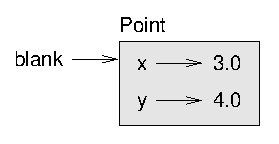
\includegraphics{figs/point.eps}}
\afterfig

The variable {\tt blank} refers to a Point object, which
contains two attributes.  Each attribute refers to a
floating-point number.

You can read the value of an attribute using the same syntax:

\beforeverb
\begin{verbatim}
>>> print blank.y
4.0
>>> x = blank.x
>>> print x
3.0
\end{verbatim}
\afterverb
%
The expression {\tt blank.x} means, ``Go to the object {\tt blank}
refers to and get the value of {\tt x}.'' In this case, we assign that
value to a variable named {\tt x}.  There is no conflict between
the variable {\tt x} and the attribute {\tt x}.

You can use dot notation as part of any expression.  For example:

\beforeverb
\begin{verbatim}
>>> print '(%g, %g)' % (blank.x, blank.y)
(3.0, 4.0)
>>> distance = math.sqrt(blank.x**2 + blank.y**2)
>>> print distance
5.0
\end{verbatim}
\afterverb
%
You can pass an instance as an argument in the usual way.
For example:

\index{instance!as argument}

\beforeverb
\begin{verbatim}
def print_point(p):
    print '(%g, %g)' % (p.x, p.y)
\end{verbatim}
\afterverb
%
\verb"print_point" takes a point as an argument and displays it in
mathematical notation.  To invoke it, you can pass {\tt blank} as
an argument:

\beforeverb
\begin{verbatim}
>>> print_point(blank)
(3.0, 4.0)
\end{verbatim}
\afterverb
%
Inside the function, {\tt p} is an alias for {\tt blank}, so if
the function modifies {\tt p}, {\tt blank} changes.

\index{aliasing}


\begin{ex}
Write a function called {\tt distance} that takes two Points
as arguments and returns the distance between them.
\end{ex}



\section{Rectangles}

Sometimes it is obvious what the attributes of an object should be,
but other times you have to make decisions.  For example, imagine you
are designing a class to represent rectangles.  What attributes would
you use to specify the location and size of a rectangle?  You can
ignore angle; to keep things simple, assume that the rectangle is
either vertical or horizontal.

\index{representation}

There are at least two possibilities: 

\begin{itemize}

\item You could specify one corner of the rectangle
(or the center), the width, and the height.

\item You could specify two opposing corners.

\end{itemize}

At this point it is hard to say whether either is better than
the other, so we'll implement the first one, just as an example.

\index{Rectangle class}
\index{class!Rectangle}

Here is the class definition:

\beforeverb
\begin{verbatim}
class Rectangle(object):
    """represent a rectangle. 
       attributes: width, height, corner.
    """
\end{verbatim}
\afterverb
%
The docstring lists the attributes:  {\tt width} and
{\tt height} are numbers; {\tt corner} is a Point object that
specifies the lower-left corner.

To represent a rectangle, you have to instantiate a Rectangle
object and assign values to the attributes:

\beforeverb
\begin{verbatim}
box = Rectangle()
box.width = 100.0
box.height = 200.0
box.corner = Point()
box.corner.x = 0.0
box.corner.y = 0.0
\end{verbatim}
\afterverb
%
The expression {\tt box.corner.x} means,
``Go to the object {\tt box} refers to and select the attribute named
{\tt corner}; then go to that object and select the attribute named
{\tt x}.''

The figure shows the state of this object:

\index{state diagram}
\index{diagram!state}
\index{object diagram}
\index{diagram!object}

\beforefig
\centerline{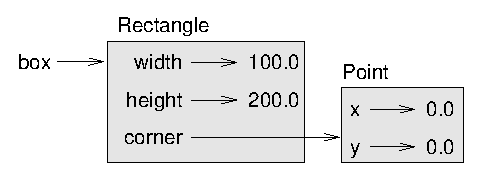
\includegraphics{figs/rectangle.eps}}
\afterfig

An object that is an attribute of another object is {\bf embedded}.

\index{embedded object}
\index{object!embedded}


\section{Instances as return values}

\index{instance!as return value}
\index{return value}

Functions can return instances.  For example, \verb"find_center"
takes a {\tt Rectangle} as an argument and returns a {\tt Point}
that contains the coordinates of the center of the {\tt Rectangle}:

\beforeverb
\begin{verbatim}
def find_center(box):
    p = Point()
    p.x = box.corner.x + box.width/2.0
    p.y = box.corner.y + box.height/2.0
    return p
\end{verbatim}
\afterverb
%
Here is an example that passes {\tt box} as an argument and assigns
the resulting Point to {\tt center}:

\beforeverb
\begin{verbatim}
>>> center = find_center(box)
>>> print_point(center)
(50.0, 100.0)
\end{verbatim}
\afterverb
%

\section{Objects are mutable}

\index{object!mutable}
\index{mutability}

You can change the state of an object by making an assignment to one of
its attributes.  For example, to change the size of a rectangle
without changing its position, you can modify the values of {\tt
width} and {\tt height}:

\beforeverb
\begin{verbatim}
box.width = box.width + 50
box.height = box.width + 100
\end{verbatim}
\afterverb
%
You can also write functions that modify objects.  For example,
\verb"grow_rectangle" takes a Rectangle object and two numbers,
{\tt dwidth} and {\tt dheight}, and adds the numbers to the
width and height of the rectangle:

\beforeverb
\begin{verbatim}
def grow_rectangle(rect, dwidth, dheight) :
    rect.width += dwidth
    rect.height += dheight
\end{verbatim}
\afterverb
%
Here is an example that demonstrates the effect:

\beforeverb
\begin{verbatim}
>>> print box.width
100.0
>>> print box.height
200.0
>>> grow_rectangle(box, 50, 100)
>>> print box.width
150.0
>>> print box.height
300.0
\end{verbatim}
\afterverb
%
Inside the function, {\tt rect} is an
alias for {\tt box}, so if the function modifies {\tt rect}, 
{\tt box} changes.

\begin{ex}
Write a function named \verb"move_rectangle" that takes
a Rectangle and two numbers named {\tt dx} and {\tt dy}.  It
should change the location of the rectangle by adding {\tt dx}
to the {\tt x} coordinate of {\tt corner} and adding {\tt dy}
to the {\tt y} coordinate of {\tt corner}.
\end{ex}


\section{Copying}

\index{aliasing}

Aliasing can make a program difficult to read because changes
in one place might have unexpected effects in another place.
It is hard to keep track of all the variables that might refer
to a given object.

\index{copying objects}
\index{object!copying}
\index{copy module}
\index{module!copy}

Copying an object is often an alternative to aliasing.
The {\tt copy} module contains a function called {\tt copy} that
can duplicate any object:

\beforeverb
\begin{verbatim}
>>> p1 = Point()
>>> p1.x = 3.0
>>> p1.y = 4.0

>>> import copy
>>> p2 = copy.copy(p1)
\end{verbatim}
\afterverb
%
{\tt p1} and {\tt p2} contain the same data, but they are
not the same Point.

\beforeverb
\begin{verbatim}
>>> print_point(p1)
(3.0, 4.0)
>>> print_point(p2)
(3.0, 4.0)
>>> p1 is p2
False
>>> p1 == p2
False
\end{verbatim}
\afterverb
%
The {\tt is} operator indicates that {\tt p1} and {\tt p2} are not the
same object, which is what we expected.  But you might have expected
{\tt ==} to yield {\tt True} because these points contain the same
data.  In that case, you will be disappointed to learn that for
instances, the default behavior of the {\tt ==} operator is the same
as the {\tt is} operator; it checks object identity, not object
equivalence.  This behavior can be changed---we'll see how later.

\index{is operator}
\index{operator!is}

If you use {\tt copy.copy} to duplicate a Rectangle, you will find
that it copies the Rectangle object but not the embedded Point.

\index{embedded object!copying}

\beforeverb
\begin{verbatim}
>>> box2 = copy.copy(box)
>>> box2 is box
False
>>> box2.corner is box.corner
True
\end{verbatim}
\afterverb
%
Here is what the object diagram looks like:

\index{state diagram}
\index{diagram!state}
\index{object diagram}
\index{diagram!object}

\vspace{0.1in}
\beforefig
\centerline{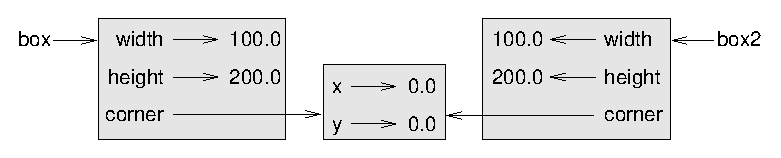
\includegraphics{figs/rectangle2.eps}}
\afterfig
\vspace{0.1in}

This operation is called a {\bf shallow copy} because it copies the
object and any references it contains, but not the embedded objects.

\index{shallow copy}
\index{copy!shallow}

For most applications, this is not what you want.  In this example,
invoking \verb"grow_rectangle" on one of the Rectangles would not
affect the other, but invoking \verb"move_rectangle" on either would
affect both!  This behavior is confusing and error-prone.

\index{deep copy}
\index{copy!deep}

Fortunately, the {\tt copy} module contains a method named {\tt
deepcopy} that copies not only the object but also 
the objects it refers to, and the objects {\em they} refer to,
and so on.
You will not be surprised to learn that this operation is
called a {\bf deep copy}.

\index{deepcopy function}
\index{function!deepcopy}

\beforeverb
\begin{verbatim}
>>> box3 = copy.deepcopy(box)
>>> box3 is box
False
>>> box3.corner is box.corner
False
\end{verbatim}
\afterverb
%
{\tt box3} and {\tt box} are completely separate objects.


\begin{ex}
Write a version of \verb"move_rectangle" that creates and
returns a new Rectangle instead of modifying the old one.
\end{ex}


\section{Debugging}
\label{hasattr}

\index{debugging}

When you start working with objects, you are likely to encounter
some new exceptions.  If you try to access an attribute
that doesn't exist, you get an {\tt AttributeError}:

\index{exception!AttributeError}
\index{AttributeError}

\beforeverb
\begin{verbatim}
>>> p = Point()
>>> print p.z
AttributeError: Point instance has no attribute 'z'
\end{verbatim}
\afterverb
%
If you are not sure what type an object is, you can ask:

\index{type function}
\index{function!type}

\beforeverb
\begin{verbatim}
>>> type(p)
<type '__main__.Point'>
\end{verbatim}
\afterverb
%
If you are not sure whether an object has a particular attribute,
you can use the built-in function {\tt hasattr}:

\index{hasattr function}
\index{function!hasattr}

\beforeverb
\begin{verbatim}
>>> hasattr(p, 'x')
True
>>> hasattr(p, 'z')
False
\end{verbatim}
\afterverb
%
The first argument can be any object; the second argument is a {\em
string} that contains the name of the attribute.


\section{Glossary}

\begin{description}

\item[class:] A user-defined type.  A class definition creates a new
class object.
\index{class}

\item[class object:] An object that contains information about a
user-defined type.  The class object can be used to create instances
of the type.
\index{class object}

\item[instance:] An object that belongs to a class.
\index{instance}

\item[attribute:] One of the named values associated with an object.
\index{attribute!instance}
\index{instance attribute}

\item[embedded (object):] An object that is stored as an attribute
of another object.
\index{embedded object}
\index{object!embedded}

\item[shallow copy:] To copy the contents of an object, including
any references to embedded objects;
implemented by the {\tt copy} function in the {\tt copy} module.
\index{shallow copy}

\item[deep copy:] To copy the contents of an object as well as any
embedded objects, and any objects embedded in them, and so on;
implemented by the {\tt deepcopy} function in the {\tt copy} module.
\index{deep copy}

\item[object diagram:] A diagram that shows objects, their
attributes, and the values of the attributes.
\index{object diagram}
\index{diagram!object}

\end{description}


\section{Exercises}

\begin{ex}
\label{canvas}

\index{Swampy}
\index{World module}
\index{module!World}

{\tt World.py}, which is part of Swampy (see Chapter~\ref{turtlechap}),
contains a class definition for a user-defined type called 
{\tt World}.  You can import it like this:

\beforeverb
\begin{verbatim}
from World import World
\end{verbatim}
\afterverb

This version of the {\tt import} statement imports the {\tt World}
class from the {\tt World} module.
The following code creates a World object and calls
the {\tt mainloop} method, which
waits for
the user.

\beforeverb
\begin{verbatim}
world = World()
world.mainloop()
\end{verbatim}
\afterverb

A window should appear with a title bar and an empty square.
We will use this window to draw Points,
Rectangles and other shapes.  
Add the following lines before calling
\verb"mainloop" and run the program again.

\index{Canvas object}
\index{object!Canvas}

\beforeverb
\begin{verbatim}
canvas = world.ca(width=500, height=500, background='white')
bbox = [[-150,-100], [150, 100]]
canvas.rectangle(bbox, outline='black', width=2, fill='green4')
\end{verbatim}
\afterverb

You should see a green rectangle with a black outline.
The first line creates a Canvas, which appears in the window
as a white square.  The Canvas object provides methods like
{\tt rectangle} for drawing various shapes.

\index{bounding box}

{\tt bbox} is a list of lists that represents the ``bounding box''
of the rectangle.  The first pair of coordinates is the lower-left
corner of the rectangle; the second pair is the upper-right corner.

You can draw a circle like this:

\beforeverb
\begin{verbatim}
canvas.circle([-25,0], 70, outline=None, fill='red')
\end{verbatim}
\afterverb

\index{Bangladesh, national flag}

The first parameter is the coordinate pair for the center of the
circle; the second parameter is the radius.

If you add this line to the program, 
the result should resemble the national flag of Bangladesh
(see \url{wikipedia.org/wiki/Gallery_of_sovereign-state_flags}).

\begin{enumerate}

\item Write a function called \verb"draw_rectangle" that takes a
  Canvas and a Rectangle as arguments and draws a
  representation of the Rectangle on the Canvas.

\item Add an attribute named {\tt color} to your Rectangle objects and
  modify \verb"draw_rectangle" so that it uses the color attribute as
  the fill color.

\item Write a function called \verb"draw_point" that takes a
  Canvas and a Point as arguments and draws a
  representation of the Point on the Canvas.

\item Define a new class called Circle with appropriate attributes and
  instantiate a few Circle objects.  Write a function called
  \verb"draw_circle" that draws circles on the canvas.

\index{Czech Republic, national flag}

\item Write a program that draws the national flag of of the Czech Republic.
Hint: you can draw a polygon like this:

\beforeverb
\begin{verbatim}
points = [[-150,-100], [150, 100], [150, -100]]
canvas.polygon(points, fill='blue')
\end{verbatim}
\afterverb

\end{enumerate}

\index{color list}
\index{available colors}

I have written a small program that lists the available colors;
you can download it from \url{thinkpython.com/code/color_list.py}.

\end{ex}



\chapter{Classes and functions}
\label{time}


\section{Time}

As another example of a user-defined type, we'll define a class called
{\tt Time} that records the time of day.  The class definition looks
like this:

\index{user-defined type}
\index{type!user-defined}
\index{Time class}
\index{class!Time}

\beforeverb
\begin{verbatim}
class Time(object):
    """represents the time of day.
       attributes: hour, minute, second"""
\end{verbatim}
\afterverb
%
We can create a new {\tt Time} object and assign
attributes for hours, minutes, and seconds:

\beforeverb
\begin{verbatim}
time = Time()
time.hour = 11
time.minute = 59
time.second = 30
\end{verbatim}
\afterverb
%
The state diagram for the {\tt Time} object looks like this:

\index{state diagram}
\index{diagram!state}
\index{object diagram}
\index{diagram!object}

\beforefig
\centerline{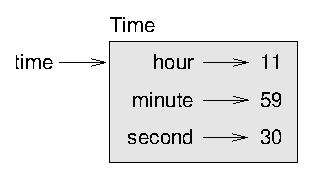
\includegraphics{figs/time.eps}}
\afterfig

\begin{ex}
\label{printtime}
Write a function called \verb"print_time" that takes a 
Time object and prints it in the form {\tt hour:minute:second}.
Hint: the format sequence \verb"'%.2d'" prints an integer using
at least two digits, including a leading zero if necessary.
\end{ex}

\begin{ex}
\label{is_after}

\index{boolean function}

Write a boolean function called \verb"is_after" that
takes two Time objects, {\tt t1} and {\tt t2}, and
returns {\tt True} if {\tt t1} follows {\tt t2} chronologically and
{\tt False} otherwise.  Challenge: don't use an {\tt if} statement.
\end{ex}


\section{Pure functions}

\index{prototype and patch}
\index{development plan!prototype and patch}

In the next few sections, we'll write two functions that add time
values.  They demonstrate two kinds of functions: pure functions and
modifiers.  They also demonstrate a development plan I'll call {\bf
  prototype and patch}, which is a way of tackling a complex problem
by starting with a simple prototype and incrementally dealing with the
complications.

Here is a simple prototype of \verb"add_time":

\beforeverb
\begin{verbatim}
def add_time(t1, t2):
    sum = Time()
    sum.hour = t1.hour + t2.hour
    sum.minute = t1.minute + t2.minute
    sum.second = t1.second + t2.second
    return sum
\end{verbatim}
\afterverb
%
The function creates a new {\tt Time} object, initializes its
attributes, and returns a reference to the new object.  This is called
a {\bf pure function} because it does not modify any of the objects
passed to it as arguments and it has no effect,
like displaying a value or getting user input, 
other than returning a value.

\index{pure function}
\index{function type!pure}

To test this function, I'll create two Time objects: {\tt start}
contains the start time of a movie, like {\em Monty Python and the
Holy Grail}, and {\tt duration} contains the run time of the movie,
which is one hour 35 minutes.

\index{Monty Python and the Holy Grail}

\verb"add_time" figures out when the movie will be done.

\beforeverb
\begin{verbatim}
>>> start = Time()
>>> start.hour = 9
>>> start.minute = 45
>>> start.second =  0

>>> duration = Time()
>>> duration.hour = 1
>>> duration.minute = 35
>>> duration.second = 0

>>> done = add_time(start, duration)
>>> print_time(done)
10:80:00
\end{verbatim}
\afterverb
%
The result, {\tt 10:80:00} might not be what you were hoping
for.  The problem is that this function does not deal with cases where the
number of seconds or minutes adds up to more than sixty.  When that
happens, we have to ``carry'' the extra seconds into the minute column
or the extra minutes into the hour column.

\index{carrying, addition with}

Here's an improved version:

\beforeverb
\begin{verbatim}
def add_time(t1, t2):
    sum = Time()
    sum.hour = t1.hour + t2.hour
    sum.minute = t1.minute + t2.minute
    sum.second = t1.second + t2.second

    if sum.second >= 60:
        sum.second -= 60
        sum.minute += 1

    if sum.minute >= 60:
        sum.minute -= 60
        sum.hour += 1

    return sum
\end{verbatim}
\afterverb
%
Although this function is correct, it is starting to get big.
We will see a shorter alternative later.


\section{Modifiers}
\label{increment}

\index{modifier}
\index{function type!modifier}

Sometimes it is useful for a function to modify the objects it gets as
parameters.  In that case, the changes are visible to the caller.
Functions that work this way are called {\bf modifiers}.

\index{increment}

{\tt increment}, which adds a given number of seconds to a {\tt Time}
object, can be written naturally as a
modifier.  Here is a rough draft:

\beforeverb
\begin{verbatim}
def increment(time, seconds):
    time.second += seconds

    if time.second >= 60:
        time.second -= 60
        time.minute += 1

    if time.minute >= 60:
        time.minute -= 60
        time.hour += 1
\end{verbatim}
\afterverb
%
The first line performs the basic operation; the remainder deals
with the special cases we saw before.

\index{special case}

Is this function correct?  What happens if the parameter {\tt seconds}
is much greater than sixty?  

In that case, it is not enough to carry
once; we have to keep doing it until {\tt time.second} is less than sixty.
One solution is to replace the {\tt if} statements with {\tt while}
statements.  That would make the function correct, but not
very efficient.

\begin{ex}
Write a correct version of {\tt increment} that
doesn't contain any loops.
\end{ex}

Anything that can be done with modifiers can also be done with pure
functions.  In fact, some programming languages only allow pure
functions.  There is some evidence that programs that use pure
functions are faster to develop and less error-prone than programs
that use modifiers.  But modifiers are convenient at times,
and functional programs tend to be less efficient.

In general, I recommend that you write pure functions whenever it is
reasonable and resort to modifiers only if there is a compelling
advantage.  This approach might be called a {\bf functional
programming style}.

\index{functional programming style}


\begin{ex}
Write a ``pure'' version of {\tt increment} that creates and returns
a new Time object rather than modifying the parameter.
\end{ex}


\section{Prototyping versus planning}
\label{prototype}

\index{prototype and patch}
\index{development plan!prototype and patch}
\index{planned development}
\index{development plan!planned}

The development plan I am demonstrating is called ``prototype and
patch.''  For each function, I wrote a prototype that performed the
basic calculation and then tested it, patching errors along the
way.

This approach can be effective, especially if you don't yet have a
deep understanding of the problem.  But incremental corrections can
generate code that is unnecessarily complicated---since it deals with
many special cases---and unreliable---since it is hard to know if you
have found all the errors.

An alternative is {\bf planned development}, in which high-level
insight into the problem can make the programming much easier.  In
this case, the insight is that a Time object is really a three-digit
number in base 60 (see \url{wikipedia.org/wiki/Sexagesimal})!  The
{\tt second} attribute is the ``ones column,'' the {\tt minute}
attribute is the ``sixties column,'' and the {\tt hour} attribute is
the ``thirty-six hundreds column.''

\index{sexagesimal}

When we wrote \verb"add_time" and {\tt increment}, we were effectively
doing addition in base 60, which is why we had to carry from one
column to the next.

\index{carrying, addition with}

This observation suggests another approach to the whole problem---we
can convert Time objects to integers and take advantage of the fact
that the computer knows how to do integer arithmetic.  

Here is a function that converts Times to integers:

\beforeverb
\begin{verbatim}
def time_to_int(time):
    minutes = time.hour * 60 + time.minute
    seconds = minutes * 60 + time.second
    return seconds
\end{verbatim}
\afterverb
%
And here is the function that converts integers to Times
(recall that {\tt divmod} divides the first argument by the second
and returns the quotient and remainder as a tuple).

\index{divmod}

\beforeverb
\begin{verbatim}
def int_to_time(seconds):
    time = Time()
    minutes, time.second = divmod(seconds, 60)
    time.hour, time.minute = divmod(minutes, 60)
    return time
\end{verbatim}
\afterverb
%
You might have to think a bit, and run some tests, to convince
yourself that these functions are correct.  One way to test them is to
check that \verb"time_to_int(int_to_time(x)) == x" for many values of
{\tt x}.  This is an example of a consistency check.

\index{consistency check}

Once you are convinced they are correct, you can use them to 
rewrite \verb"add_time":

\beforeverb
\begin{verbatim}
def add_time(t1, t2):
    seconds = time_to_int(t1) + time_to_int(t2)
    return int_to_time(seconds)
\end{verbatim}
\afterverb
%
This version is shorter than the original, and easier to verify.

\begin{ex}
Rewrite {\tt increment} using \verb"time_to_int" and \verb"int_to_time".
\end{ex}

In some ways, converting from base 60 to base 10 and back is harder
than just dealing with times.  Base conversion is more abstract; our
intuition for dealing with time values is better.

But if we have the insight to treat times as base 60 numbers and make
the investment of writing the conversion functions (\verb"time_to_int"
and \verb"int_to_time"), we get a program that is shorter, easier to
read and debug, and more reliable.

It is also easier to add features later.  For example, imagine
subtracting two Times to find the duration between them.  The
na\"{\i}ve approach would be to implement subtraction with borrowing.
Using the conversion functions would be easier and more likely to be
correct.

\index{subtraction with borrowing}
\index{borrowing, subtraction with}
\index{generalization}

Ironically, sometimes making a problem harder (or more general) makes it
easier (because there are fewer special cases and fewer opportunities
for error).


\section{Debugging}
\index{debugging}

A Time object is well-formed if the values of {\tt minutes} and {\tt
seconds} are between 0 and 60 (including 0 but not 60) and if 
{\tt hours} is positive.  {\tt hours} and {\tt minutes} should be
integral values, but we might allow {\tt seconds} to have a
fraction part.

\index{invariant}

These kind of requirements are called {\bf invariants} because
they should always be true.  To put it a different way, if they
are not true, then something has gone wrong.

Writing code to check your invariants can help you detect errors
and find their causes.  For example, you might have a function
like \verb"valid_time" that takes a Time object and returns
{\tt False} if it violates an invariant:

\beforeverb
\begin{verbatim}
def valid_time(time):
    if time.hours < 0 or time.minutes < 0 or time.seconds < 0:
        return False
    if time.minutes >= 60 or time.seconds >= 60:
        return False
    return True
\end{verbatim}
\afterverb
%
Then at the beginning of each function you could check the
arguments to make sure they are valid:

\index{raise statement}
\index{statement!raise}

\beforeverb
\begin{verbatim}
def add_time(t1, t2):
    if not valid_time(t1) or not valid_time(t2):
        raise ValueError, 'invalid Time object in add_time'
    seconds = time_to_int(t1) + time_to_int(t2)
    return int_to_time(seconds)
\end{verbatim}
\afterverb
%
Or you could use an {\tt assert} statement, which checks a given invariant
and raises an exception if it fails:

\index{assert statement}
\index{statement!assert}

\beforeverb
\begin{verbatim}
def add_time(t1, t2):
    assert valid_time(t1) and valid_time(t2)
    seconds = time_to_int(t1) + time_to_int(t2)
    return int_to_time(seconds)
\end{verbatim}
\afterverb
%
{\tt assert} statements are useful because they distinguish
code that deals with normal conditions from code
that checks for errors.


\section{Glossary}

\begin{description}

\item[prototype and patch:] A development plan that involves
writing a rough draft of a program, testing, and correcting errors as
they are found.
\index{prototype and patch}

\item[planned development:] A development plan that involves
high-level insight into the problem and more planning than incremental
development or prototype development.
\index{planned development}

\item[pure function:] A function that does not modify any of the objects it
receives as arguments.  Most pure functions are fruitful.
\index{pure function}

\item[modifier:] A function that changes one or more of the objects it
receives as arguments.  Most modifiers are fruitless.
\index{modifier}

\item[functional programming style:] A style of program design in which the
majority of functions are pure.
\index{functional programming style}

\item[invariant:] A condition that should always be true during the
execution of a program.
\index{invariant}

\end{description}


\section{Exercises}

\begin{ex}
Write a function called \verb"mul_time" that takes a Time object
and a number and returns a new Time object that contains
the product of the original Time and the number.

Then use \verb"mul_time" to write a function that takes a Time
object that represents the finishing time in a race, and a number
that represents the distance, and returns a Time object that represents
the average pace (time per mile).

\index{running pace}

\end{ex}

\begin{ex}

\index{Date class}
\index{class!Date}

Write a class definition for a Date object that has attributes {\tt
  day}, {\tt month} and {\tt year}.  Write a function called
\verb"increment_date" that takes a Date object, {\tt date} and an
integer, {\tt n}, and returns a new Date object that
represents the day {\tt n} days after {\tt date}.  Hint:
``Thirty days hath September...''  Challenge: does your function
deal with leap years correctly?  See \url{wikipedia.org/wiki/Leap_year}

\end{ex}


\begin{ex}

\index{datetime module}
\index{module!datetime}

The {\tt datetime} module provides {\tt date} and {\tt time} objects
that are similar to the Date and Time objects in this chapter, but
they provide a rich set of methods and operators.  Read the
documentation at \url{docs.python.org/lib/datetime-date.html}.

\begin{enumerate}

\item Use the {\tt datetime} module to write a program that
gets the current date and prints the day of the week.

\index{birthday}

\item Write a program that takes a birthday as input
and prints the user's age and the number of days, hours,
minutes and seconds until their next birthday.
\end{enumerate}

\end{ex}


\chapter{Classes and methods}


\section{Object-oriented features}

\index{object-oriented programming}

Python is an {\bf object-oriented programming language}, which means
that it provides features that support object-oriented
programming.

It is not easy to define object-oriented programming, but we have
already seen some of its characteristics:

\begin{itemize}

\item Programs are made up of object definitions and function
definitions, and most of the computation is expressed in terms
of operations on objects.

\item Each object definition corresponds to some object or concept
in the real world, and the functions that operate on that object
correspond to the ways real-world objects interact.

\end{itemize}

For example, the {\tt Time} class defined in Chapter~\ref{time}
corresponds to the way people record the time of day, and the
functions we defined correspond to the kinds of things people do with
times.  Similarly, the {\tt Point} and {\tt Rectangle} classes
correspond to the mathematical concepts of a point and a rectangle.

So far, we have not taken advantage of the features Python provides to
support object-oriented programming.  These
features are not strictly necessary; most of them provide
alternative syntax for things we have already done.  But in many cases,
the alternative is more concise and more accurately conveys the
structure of the program.

For example, in the {\tt Time} program, there is no obvious
connection between the class definition and the function definitions
that follow.  With some examination, it is apparent that every function
takes at least one {\tt Time} object as an argument.

\index{method}
\index{function}

This observation is the motivation for {\bf methods}; a method is
a function that is associated with a particular class.
We have seen methods for strings, lists, dictionaries and tuples.
In this chapter, we will define methods for user-defined types.

\index{syntax}
\index{semantics}

Methods are semantically the same as functions, but there are
two syntactic differences:

\begin{itemize}

\item Methods are defined inside a class definition in order
to make the relationship between the class and the method explicit.

\item The syntax for invoking a method is different from the
syntax for calling a function.

\end{itemize}

In the next few sections, we will take the functions from the previous
two chapters and transform them into methods.  This transformation is
purely mechanical; you can do it simply by following a sequence of
steps.  If you are comfortable converting from one form to another,
you will be able to choose the best form for whatever you are doing.


\section{Printing objects}
\label{print_time}

\index{object!printing}

In Chapter~\ref{time}, we defined a class named
{\tt Time} and in Exercise~\ref{printtime}, you 
wrote a function named \verb"print_time":

\beforeverb
\begin{verbatim}
class Time(object):
    """represents the time of day.
       attributes: hour, minute, second"""

def print_time(time):
    print '%.2d:%.2d:%.2d' % (time.hour, time.minute, time.second)
\end{verbatim}
\afterverb
%
To call this function, you have to pass a {\tt Time} object as an
argument:

\beforeverb
\begin{verbatim}
>>> start = Time()
>>> start.hour = 9
>>> start.minute = 45
>>> start.second = 00
>>> print_time(start)
09:45:00
\end{verbatim}
\afterverb
%
To make \verb"print_time" a method, all we have to do is
move the function definition inside the class definition.  Notice
the change in indentation.

\index{indentation}

\beforeverb
\begin{verbatim}
class Time(object):
    def print_time(time):
        print '%.2d:%.2d:%.2d' % (time.hour, time.minute, time.second)
\end{verbatim}
\afterverb
%
Now there are two ways to call \verb"print_time".  The first
(and less common) way is to use function syntax:

\index{function syntax}
\index{dot notation}


\beforeverb
\begin{verbatim}
>>> Time.print_time(start)
09:45:00
\end{verbatim}
\afterverb
%
In this use of dot notation, {\tt Time} is the name of the class,
and \verb"print_time" is the name of the method.  {\tt start} is
passed as a parameter.

The second (and more concise) way is to use method syntax:

\index{method syntax}

\beforeverb
\begin{verbatim}
>>> start.print_time()
09:45:00
\end{verbatim}
\afterverb
%
In this use of dot notation, \verb"print_time" is the name of the
method (again), and {\tt start} is the object the method is
invoked on, which is called the {\bf subject}.  Just as the
subject of a sentence is what the sentence is about, the subject
of a method invocation is what the method is about.

\index{subject}

Inside the method, the subject is assigned to the first
parameter, so in this case {\tt start} is assigned
to {\tt time}.

\index{self (parameter name)}
\index{parameter!self}

By convention, the first parameter of a method is
called {\tt self}, so it would be more common to write
\verb"print_time" like this:

\beforeverb
\begin{verbatim}
class Time(object):
    def print_time(self):
        print '%.2d:%.2d:%.2d' % (self.hour, self.minute, self.second)
\end{verbatim}
\afterverb
%
The reason for this convention is an implicit metaphor:

\index{metaphor, method invocation}

\begin{itemize}

\item The syntax for a function call, \verb"print_time(start)",
  suggests that the function is the active agent.  It says something
  like, ``Hey \verb"print_time"!  Here's an object for you to print.''

\item In object-oriented programming, the objects are the active
  agents.  A method invocation like \verb"start.print_time()" says
  ``Hey {\tt start}!  Please print yourself.''

\end{itemize}

This change in perspective might be more polite, but it is not obvious
that it is useful.  In the examples we have seen so far, it may not
be.  But sometimes shifting responsibility from the functions onto the
objects makes it possible to write more versatile functions, and makes
it easier to maintain and reuse code.

\begin{ex}
\label{convert}
Rewrite \verb"time_to_int"
(from Section~\ref{prototype}) as a method.  It is probably not
appropriate to rewrite \verb"int_to_time" as a method; it's not
clear what object you would invoke it on!
\end{ex}


\section{Another example}

\index{increment}

Here's a version of {\tt increment} (from Section~\ref{increment})
rewritten as a method:

\beforeverb
\begin{verbatim}
# inside class Time:

    def increment(self, seconds):
        seconds += self.time_to_int()
        return int_to_time(seconds)
\end{verbatim}
\afterverb
%
This version assumes that \verb"time_to_int" is written
as a method, as in Exercise~\ref{convert}.  Also, note that
it is a pure function, not a modifier.

Here's how you would invoke {\tt increment}:

\beforeverb
\begin{verbatim}
>>> start.print_time()
09:45:00
>>> end = start.increment(1337)
>>> end.print_time()
10:07:17
\end{verbatim}
\afterverb
%
The subject, {\tt start}, gets assigned to the first parameter,
{\tt self}.  The argument, {\tt 1337}, gets assigned to the
second parameter, {\tt seconds}.

This mechanism can be confusing, especially if you make an error.
For example, if you invoke {\tt increment} with two arguments, you
get:

\index{exception!TypeError}
\index{TypeError}

\beforeverb
\begin{verbatim}
>>> end = start.increment(1337, 460)
TypeError: increment() takes exactly 2 arguments (3 given)
\end{verbatim}
\afterverb
%
The error message is initially confusing, because there are
only two arguments in parentheses.  But the subject is also
considered an argument, so all together that's three.


\section{A more complicated example}

\verb"is_after" (from Exercise~\ref{is_after}) is slightly more complicated
because it takes two Time objects as parameters.  In this case it is
conventional to name the first parameter {\tt self} and the second
parameter {\tt other}:

\index{other (parameter name)}
\index{parameter!other}

\beforeverb
\begin{verbatim}
# inside class Time:

    def is_after(self, other):
        return self.time_to_int() > other.time_to_int()
\end{verbatim}
\afterverb
%
To use this method, you have to invoke it on one object and pass
the other as an argument:

\beforeverb
\begin{verbatim}
>>> end.is_after(start)
True
\end{verbatim}
\afterverb
%
One nice thing about this syntax is that it almost reads
like English: ``end is after start?''


\section{The init method}

\index{init method}
\index{method!init}

The init method (short for ``initialization'') is
a special method that gets invoked when an object is instantiated.  
Its full name is \verb"__init__" (two underscore characters,
followed by {\tt init}, and then two more underscores).  An
init method for the {\tt Time} class might look like this:

\beforeverb
\begin{verbatim}
# inside class Time:

    def __init__(self, hour=0, minute=0, second=0):
        self.hour = hour
        self.minute = minute
        self.second = second
\end{verbatim}
\afterverb
%
It is common for the parameters of \verb"__init__"
to have the same names as the attributes.  The statement

\beforeverb
\begin{verbatim}
        self.hour = hour
\end{verbatim}
\afterverb
%
stores the value of the parameter {\tt hour} as an attribute
of {\tt self}.

\index{optional parameter}
\index{parameter!optional}
\index{default value}
\index{override}

The parameters are optional, so if you call {\tt Time} with
no arguments, you get the default values.

\beforeverb
\begin{verbatim}
>>> time = Time()
>>> time.print_time()
00:00:00
\end{verbatim}
\afterverb
%
If you provide one argument, it overrides {\tt hour}:

\beforeverb
\begin{verbatim}
>>> time = Time (9)
>>> time.print_time()
09:00:00
\end{verbatim}
\afterverb
%
If you provide two arguments, they override {\tt hour} and
{\tt minute}.

\beforeverb
\begin{verbatim}
>>> time = Time(9, 45)
>>> time.print_time()
09:45:00
\end{verbatim}
\afterverb
%
And if you provide three arguments, they override all three
default values.


\begin{ex}
\index{Point class}
\index{class!Point}

Write an init method for the {\tt Point} class that takes
{\tt x} and {\tt y} as optional parameters and assigns
them to the corresponding attributes.
\end{ex}


\section{The {\tt \_\_str\_\_} method}

\index{str method@\_\_str\_\_ method}
\index{method!\_\_str\_\_}

\verb"__str__" is a special method, like \verb"__init__",
that is supposed to return a string representation of an object.

\index{string representation}

For example, here is a {\tt str} method for Time objects:

\beforeverb
\begin{verbatim}
# inside class Time:

    def __str__(self):
        return '%.2d:%.2d:%.2d' % (self.hour, self.minute, self.second)
\end{verbatim}
\afterverb
%
When you {\tt print} an object, Python invokes the {\tt str} method:

\index{print statement}
\index{statement!print}

\beforeverb
\begin{verbatim}
>>> time = Time(9, 45)
>>> print time
09:45:00
\end{verbatim}
\afterverb
%
When I write a new class, I almost always start by writing 
\verb"__init__", which makes it easier to instantiate objects, and 
\verb"__str__", which is useful for debugging.


\begin{ex}
Write a {\tt str} method for the {\tt Point} class.  Create
a Point object and print it.
\end{ex}


\section{Operator overloading}
\label{operator overloading}

By defining other special methods, you can specify the behavior
of operators on user-defined types.  For example, if you define
a method named \verb"__add__" for the {\tt Time} class, you can use the
{\tt +} operator on Time objects.

Here is what the definition might look like:

\index{add method}
\index{method!add}

\beforeverb
\begin{verbatim}
# inside class Time:

    def __add__(self, other):
        seconds = self.time_to_int() + other.time_to_int()
        return int_to_time(seconds)
\end{verbatim}
\afterverb
%
And here is how you could use it:

\beforeverb
\begin{verbatim}
>>> start = Time(9, 45)
>>> duration = Time(1, 35)
>>> print start + duration
11:20:00
\end{verbatim}
\afterverb
%
When you apply the {\tt +} operator to Time objects, Python invokes
\verb"__add__".  When you print the result, Python invokes 
\verb"__str__".  So there is quite a lot happening behind the scenes!

\index{operator overloading}

Changing the behavior of an operator so that it works with
user-defined types is called {\bf operator overloading}.  For every
operator in Python there is a corresponding special method, like 
\verb"__add__".  For more details, see
\url{docs.python.org/ref/specialnames.html}.

\begin{ex}
Write an {\tt add} method for the Point class.  
\end{ex}


\section{Type-based dispatch}

In the previous section we added two Time objects, but you
also might want to add an integer to a Time object.  The
following is a version of \verb"__add__"
that checks the type of {\tt other} and invokes either
\verb"add_time" or {\tt increment}:

\beforeverb
\begin{verbatim}
# inside class Time:

    def __add__(self, other):
        if isinstance(other, Time):
            return self.add_time(other)
        else:
            return self.increment(other)

    def add_time(self, other):
        seconds = self.time_to_int() + other.time_to_int()
        return int_to_time(seconds)

    def increment(self, seconds):
        seconds += self.time_to_int()
        return int_to_time(seconds)
\end{verbatim}
\afterverb
%
The built-in function {\tt isinstance} takes a value and a
class object, and returns {\tt True} if the value is an instance
of the class.

\index{isinstance function}
\index{function!isinstance}

If {\tt other} is a Time object, \verb"__add__" invokes
\verb"add_time".  Otherwise it assumes that the parameter
is a number and invokes {\tt increment}.  This operation is
called a {\bf type-based dispatch} because it dispatches the
computation to different methods based on the type of the
arguments.

\index{type-based dispatch}
\index{dispatch, type-based}

Here are examples that use the {\tt +} operator with different
types:

\beforeverb
\begin{verbatim}
>>> start = Time(9, 45)
>>> duration = Time(1, 35)
>>> print start + duration
11:20:00
>>> print start + 1337
10:07:17
\end{verbatim}
\afterverb
%
Unfortunately, this implementation of addition is not commutative.
If the integer is the first operand, you get

\index{commutativity}

\beforeverb
\begin{verbatim}
>>> print 1337 + start
TypeError: unsupported operand type(s) for +: 'int' and 'instance'
\end{verbatim}
\afterverb
%
The problem is, instead of asking the Time object to add an integer,
Python is asking an integer to add a Time object, and it doesn't know
how to do that.  But there is a clever solution for this problem: the
special method \verb"__radd__", which stands for ``right-side add.''
This method is invoked when a Time object appears on the right side of
the {\tt +} operator.  Here's the definition:

\index{radd method}
\index{method!radd}

\beforeverb
\begin{verbatim}
# inside class Time:

    def __radd__(self, other):
        return self.__add__(other)
\end{verbatim}
\afterverb
%
And here's how it's used:

\beforeverb
\begin{verbatim}
>>> print 1337 + start
10:07:17
\end{verbatim}
\afterverb
%

\begin{ex}
Write an {\tt add} method for Points that works with either a
Point object or a tuple:  

\begin{itemize}

\item If the second operand is a Point, the method should return a new
Point whose $x$ coordinate is the sum of the $x$ coordinates of the
operands, and likewise for the $y$ coordinates.

\item If the second operand is a tuple, the method should add the
first element of the tuple to the $x$ coordinate and the second
element to the $y$ coordinate, and return a new Point with the result. 

\end{itemize}

\end{ex}

\section{Polymorphism}

Type-based dispatch is useful when it is necessary, but (fortunately)
it is not always necessary.  Often you can avoid it by writing functions
that work correctly for arguments with different types.

\index{type-based dispatch}
\index{dispatch!type-based}

Many of the functions we wrote for strings will actually
work for any kind of sequence.
For example, in Section~\ref{histogram}
we used {\tt histogram} to count the number of times each letter
appears in a word.

\beforeverb
\begin{verbatim}
def histogram(s):
    d = dict()
    for c in s:
        if c not in d:
            d[c] = 1
        else:
            d[c] = d[c]+1
    return d
\end{verbatim}
\afterverb
%
This function also works for lists, tuples, and even dictionaries,
as long as the elements of {\tt s} are hashable, so they can be used
as keys in {\tt d}.

\beforeverb
\begin{verbatim}
>>> t = ['spam', 'egg', 'spam', 'spam', 'bacon', 'spam']
>>> histogram(t)
{'bacon': 1, 'egg': 1, 'spam': 4}
\end{verbatim}
\afterverb
%
Functions that can work with several types are called {\bf polymorphic}.
Polymorphism can facilitate code reuse.  For example, the built-in
function {\tt sum}, which adds the elements of a sequence, works
as long as the elements of the sequence support addition.

\index{polymorphism}

Since Time objects provide an {\tt add} method, they work
with {\tt sum}:

\beforeverb
\begin{verbatim}
>>> t1 = Time(7, 43)
>>> t2 = Time(7, 41)
>>> t3 = Time(7, 37)
>>> total = sum([t1, t2, t3])
>>> print total
23:01:00
\end{verbatim}
\afterverb
%
In general, if all of the operations inside a function 
work with a given type, then the function works with that type.

The best kind of polymorphism is the unintentional kind, where
you discover that a function you already wrote can be
applied to a type you never planned for.


\section{Debugging}
\index{debugging}

It is legal to add attributes to objects at any point in the execution
of a program, but if you are a stickler for type theory, it is a
dubious practice to have objects of the same type with different
attribute sets.  It is usually a good idea to
initialize all of an objects attributes in the init method.

\index{init method}
\index{attribute!initializing}

If you are not sure whether an object has a particular attribute, you
can use the built-in function {\tt hasattr} (see Section~\ref{hasattr}).

\index{hasattr function}
\index{function!hasattr}
\index{dict attribute@\_\_dict\_\_ attribute}
\index{attribute!\_\_dict\_\_}

Another way to access the attributes of an object is through the
special attribute \verb"__dict__", which is a dictionary that maps
attribute names (as strings) and values:

\beforeverb
\begin{verbatim}
>>> p = Point(3, 4)
>>> print p.__dict__
{'y': 4, 'x': 3}
\end{verbatim}
\afterverb
%
For purposes of debugging, you might find it useful to keep this
function handy:

\beforeverb
\begin{verbatim}
def print_attributes(obj):
    for attr in obj.__dict__:
        print attr, getattr(obj, attr)
\end{verbatim}
\afterverb
%
\verb"print_attributes" traverses the items in the object's dictionary
and prints each attribute name and its corresponding value.

\index{traversal!dictionary}
\index{dictionary!traversal}

The built-in function {\tt getattr} takes an object and an attribute
name (as a string) and returns the attribute's value.

\index{getattr function}
\index{function!getattr}


\section{Glossary}

\begin{description}

\item[object-oriented language:] A language that provides features,
  such as user-defined classes and method syntax, that facilitate
  object-oriented programming.
\index{object-oriented language}

\item[object-oriented programming:] A style of programming in which
data and the operations that manipulate it are organized into classes
and methods.
\index{object-oriented programming}

\item[method:] A function that is defined inside a class definition and
is invoked on instances of that class.
\index{method}

\item[subject:] The object a method is invoked on.
\index{subject}

\item[operator overloading:] Changing the behavior of an operator like
{\tt +} so it works with a user-defined type.
\index{overloading}
\index{operator!overloading}

\item[type-based dispatch:] A programming pattern that checks the type
of an operand and invokes different functions for different types.
\index{type-based dispatch}

\item[polymorphic:] Pertaining to a function that can work with more
  than one type.  

\index{polymorphism}

\end{description}

\section{Exercises}

\begin{ex}

\index{default value!avoiding mutable}
\index{mutable object, as default value}
\index{worst bug}
\index{bug!worst}

This exercise is a cautionary tale about one of the most
common, and difficult to find, errors in Python.

\begin{enumerate}

\index{Kangaroo class}
\index{class!Kangaroo}

\item Write a definition for a class named {\tt Kangaroo} with the following
methods:

\begin{enumerate}

\item An \verb"__init__" method that initializes an attribute named 
\verb"pouch_contents" to an empty list.

\item A method named \verb"put_in_pouch" that takes an object
of any type and adds it to \verb"pouch_contents".

\item A \verb"__str__" method that returns a string representation
of the Kangaroo object and the contents of the pouch.

\end{enumerate}
%
Test your code 
by creating two {\tt Kangaroo} objects, assigning them to variables
named {\tt kanga} and {\tt roo}, and then adding {\tt roo} to the
contents of {\tt kanga}'s pouch.

\item Download \url{thinkpython.com/code/BadKangaroo.py}.  It contains
a solution to the previous problem with one big, nasty bug.
Find and fix the bug.

If you get stuck, you can download
\url{thinkpython.com/code/GoodKangaroo.py}, which explains the
problem and demonstrates a solution.

\index{aliasing}
\index{embedded object}
\index{object!embedded}

\end{enumerate}


\end{ex}




\begin{ex}

\index{Visual module}
\index{module!Visual}
\index{vpython module}
\index{module!vpython}

Visual is a Python module that provides 3-D graphics.  It is
not always included in a Python installation, so you might have
to install it from your software repository or, if it's not there,
from \url{vpython.org}.

The following example creates a 3-D space that is 256 units
wide, long and high, and sets the ``center'' to be the
point $(128, 128, 128)$.  Then it draws a blue sphere.

\beforeverb
\begin{verbatim}
from visual import *

scene.range = (256, 256, 256)
scene.center = (128, 128, 128)

color = (0.1, 0.1, 0.9)          # mostly blue
sphere(pos=scene.center, radius=128, color=color)
\end{verbatim}
\afterverb

{\tt color} is an RGB tuple; that is, the elements are Red-Green-Blue
levels between 0.0 and 1.0 (see
\url{wikipedia.org/wiki/RGB_color_model}).

If you run this code, you should see a window with a black
background and a blue sphere.  If you drag the middle button
up and down, you can zoom in and out.  You can also rotate
the scene by dragging the right button, but with only one
sphere in the world, it is hard to tell the difference.

The following loop creates a cube of spheres:

\beforeverb
\begin{verbatim}
t = range(0, 256, 51)
for x in t:
    for y in t:
        for z in t:
            pos = x, y, z
            sphere(pos=pos, radius=10, color=color)
\end{verbatim}
\afterverb

\begin{enumerate}

\item Put this code in a script and make sure it works for
you.

\item Modify the program so that each sphere in the cube
has the color that corresponds to its position in RGB space.
Notice that the coordinates are in the range 0--255, but
the RGB tuples are in the range 0.0--1.0.

\index{color list}
\index{available colors}

\item Download \url{thinkpython.com/code/color_list.py}
and use the function \verb"read_colors" to generate a list
of the available colors on your system, their names and
RGB values.  For each named color draw a sphere in the
position that corresponds to its RGB values.



\end{enumerate}

You can see my solution at \url{thinkpython.com/code/color_space.py}.

\end{ex}


\chapter{Inheritance}

In this chapter we will develop classes to represent playing cards,
decks of cards, and poker hands.  If you don't play poker, you can
read about it at \url{wikipedia.org/wiki/Poker}, but you don't have
to; I'll tell you what you need to know for the exercises.

\index{playing card, Anglo-American}
\index{card, playing}
\index{poker}

If you are not familiar with Anglo-American playing cards,
you can read about them at \url{wikipedia.org/wiki/Playing_cards}.


\section{Card objects}

There are fifty-two cards in a deck, each of which belongs to one of
four suits and one of thirteen ranks.  The suits are Spades, Hearts,
Diamonds, and Clubs (in descending order in bridge).  The ranks are
Ace, 2, 3, 4, 5, 6, 7, 8, 9, 10, Jack, Queen, and King.  Depending on
the game that you are playing, an Ace may be higher than King
or lower than 2.

\index{rank}
\index{suit}

If we want to define a new object to represent a playing card, it is
obvious what the attributes should be: {\tt rank} and
{\tt suit}.  It is not as obvious what type the attributes
should be.  One possibility is to use strings containing words like
\verb"'Spade'" for suits and \verb"'Queen'" for ranks.  One problem with
this implementation is that it would not be easy to compare cards to
see which had a higher rank or suit.

\index{encode}
\index{encrypt}
\index{map to}
\index{representation}

An alternative is to use integers to {\bf encode} the ranks and suits.
In this context, ``encode'' means that we are going to define a mapping
between numbers and suits, or between numbers and ranks.  This
kind of encoding is not meant to be a secret (that
would be ``encryption'').

For example, this table shows the suits and the corresponding integer
codes:

\beforefig
\begin{tabular}{l c l}
Spades & $\mapsto$ & 3 \\
Hearts & $\mapsto$ & 2 \\
Diamonds & $\mapsto$ & 1 \\
Clubs & $\mapsto$ & 0
\end{tabular}
\afterfig

This code makes it easy to compare cards; because higher suits map to
higher numbers, we can compare suits by comparing their codes.

The mapping for ranks is fairly obvious; each of the numerical ranks
maps to the corresponding integer, and for face cards:

\beforefig
\begin{tabular}{l c l}
Jack & $\mapsto$ & 11 \\
Queen & $\mapsto$ & 12 \\
King & $\mapsto$ & 13 \\
\end{tabular}
\afterfig

I am using the $\mapsto$ symbol to make is clear that these mappings
are not part of the Python program.  They are part of the program
design, but they don't appear explicitly in the code.

\index{Card class}
\index{class!Card}

The class definition for {\tt Card} looks like this:

\beforeverb
\begin{verbatim}
class Card(object):
    """represents a standard playing card."""

    def __init__(self, suit=0, rank=2):
        self.suit = suit
        self.rank = rank
\end{verbatim}
\afterverb
%
As usual, the init method takes an optional
parameter for each attribute.  The default card is
the 2 of Clubs.

\index{init method}
\index{method!init}

To create a Card, you call {\tt Card} with the
suit and rank of the card you want.

\beforeverb
\begin{verbatim}
queen_of_diamonds = Card(1, 12)
\end{verbatim}
\afterverb
%


\section{Class attributes}

\index{class attribute}
\index{attribute!class}

In order to print Card objects in a way that people can easily
read, we need a mapping from the integer codes to the corresponding
ranks and suits.  A natural way to
do that is with lists of strings.  We assign these lists to {\bf class
attributes}:

\beforeverb
\begin{verbatim}
# inside class Card:

    suit_names = ['Clubs', 'Diamonds', 'Hearts', 'Spades']
    rank_names = [None, 'Ace', '2', '3', '4', '5', '6', '7', 
              '8', '9', '10', 'Jack', 'Queen', 'King']

    def __str__(self):
        return '%s of %s' % (Card.rank_names[self.rank],
                             Card.suit_names[self.suit])
\end{verbatim}
\afterverb
%
Variables like \verb"suit_names" and \verb"rank_names", which are
defined inside a class but outside of any method, are called
class attributes because they are associated with the class object 
{\tt Card}.

\index{instance attribute}
\index{attribute!instance}

This term distinguished them from variables like {\tt suit} and {\tt
  rank}, which are called {\bf instance attributes} because they are
associated with a particular instance.

\index{dot notation}

Both kinds of attribute are accessed using dot notation.  For
example, in \verb"__str__", {\tt self} is a Card object,
and {\tt self.rank} is its rank.  Similarly, {\tt Card}
is a class object, and \verb"Card.rank_names" is a
list of strings associated with the class.

Every card has its own {\tt suit} and {\tt rank}, but there
is only one copy of \verb"suit_names" and \verb"rank_names".

Putting it all together, the expression
\verb"Card.rank_names[self.rank]" means ``use the attribute {\tt rank}
from the object {\tt self} as an index into the list \verb"rank_names"
from the class {\tt Card}, and select the appropriate string.''

The first element of \verb"rank_names" is {\tt None} because there
is no card with rank zero.  By including {\tt None} as a place-keeper,
we get a mapping with the nice property that the index 2 maps to the
string \verb"'2'", and so on.  To avoid this tweak, we could have
used a dictionary instead of a list.

With the methods we have so far, we can create and print cards:

\beforeverb
\begin{verbatim}
>>> card1 = Card(2, 11)
>>> print card1
Jack of Hearts
\end{verbatim}
\afterverb
%
Here is a diagram that shows the {\tt Card} class object
and one Card instance:

\index{state diagram}
\index{diagram!state}
\index{object diagram}
\index{diagram!object}

\beforefig
\centerline{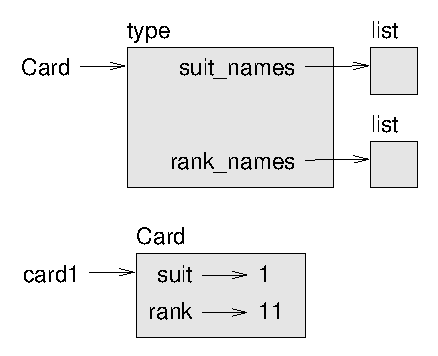
\includegraphics{figs/card1.eps}}
\afterfig

{\tt Card} is a class object, so it has type {\tt type}.  {\tt
card1} has type {\tt Card}.  (To save space, I didn't draw the
contents of \verb"suit_names" and \verb"rank_names").


\section{Comparing cards}
\label{comparecard}

\index{operator!conditional}
\index{conditional operator}

For built-in types, there are conditional operators
({\tt <}, {\tt >}, {\tt ==}, etc.)
that compare
values and determine when one is greater than, less than, or equal to
another.  For user-defined types, we can override the behavior of
the built-in operators by providing a method named
\verb"__cmp__".  

\verb"__cmp__" takes two parameters, {\tt self} and {\tt other},
and returns a positive number if the first object is greater, a
negative number if the second object is greater, and 0 if they are
equal to each other.

\index{override}
\index{operator overloading}

The correct ordering for cards is not obvious.
For example, which
is better, the 3 of Clubs or the 2 of Diamonds?  One has a higher
rank, but the other has a higher suit.  In order to compare
cards, you have to decide whether rank or suit is more important.

The answer might depend on what game you are playing, but to keep
things simple, we'll make the arbitrary choice that suit is more
important, so all of the Spades outrank all of the Diamonds,
and so on.

\index{cmp method@\_\_cmp\_\_ method}
\index{method!\_\_cmp\_\_}

With that decided, we can write \verb"__cmp__":

\beforeverb
\begin{verbatim}
# inside class Card:

    def __cmp__(self, other):
        # check the suits
        if self.suit > other.suit: return 1
        if self.suit < other.suit: return -1

        # suits are the same... check ranks
        if self.rank > other.rank: return 1
        if self.rank < other.rank: return -1

        # ranks are the same... it's a tie
        return 0    
\end{verbatim}
\afterverb
%
You can write this more concisely using tuple comparison:

\index{tuple!comparison}
\index{comparison!tuple}

\beforeverb
\begin{verbatim}
# inside class Card:

    def __cmp__(self, other):
        t1 = self.suit, self.rank
        t2 = other.suit, other.rank
        return cmp(t1, t2)
\end{verbatim}
\afterverb
%
The built-in function {\tt cmp} has the same interface as
the method \verb"__cmp__": it takes two values and returns
a positive number if the first is larger, a negative number
if the second is larger, and 0 if they are equal.

\index{cmp function}
\index{function!cmp}


\begin{ex}
Write a \verb"__cmp__" method for Time objects.  Hint: you
can use tuple comparison, but you also might consider using
integer subtraction.

%    def __cmp__(self, other):
%        return time_to_int(self) - time_to_int(other)

%If {\tt self} is later than {\tt other}, the result is
%a positive number.  If {\tt other} is later, the result
%is negative.  And if {\tt self} and {\tt other} are equal
%(but not necessarily identical)
%the result is zero.

\end{ex}


\section{Decks}
\index{list!of objects}
\index{deck, playing cards}

Now that we have Cards, the next step is to define Decks.  Since a
deck is made up of cards, it is natural for each Deck to contain a
list of cards as an attribute.

\index{init method}
\index{method!init}

The following is a class definition for {\tt Deck}.  The
init method creates the attribute {\tt cards} and generates
the standard set of fifty-two cards:

\index{composition}
\index{loop!nested}

\index{Deck class}
\index{class!Deck}

\beforeverb
\begin{verbatim}
class Deck(object):

    def __init__(self):
        self.cards = []
        for suit in range(4):
            for rank in range(1, 14):
                card = Card(suit, rank)
                self.cards.append(card)
\end{verbatim}
\afterverb
%
The easiest way to populate the deck is with a nested loop.  The outer
loop enumerates the suits from 0 to 3.  The inner loop enumerates the
ranks from 1 to 13.  Each iteration
creates a new Card with the current suit and rank,
and appends it to {\tt self.cards}.

\index{append method}
\index{method!append}


\section{Printing the deck}
\label{printdeck}

\index{str method@\_\_str\_\_ method}
\index{method!\_\_str\_\_}

Here is a \verb"__str__" method for {\tt Deck}:

\beforeverb
\begin{verbatim}
#inside class Deck:

    def __str__(self):
        res = []
        for card in self.cards:
            res.append(str(card))
        return '\n'.join(res)
\end{verbatim}
\afterverb
%
This method demonstrates an efficient way to accumulate a large
string: building a list of strings and then using {\tt join}.
The built-in function {\tt str} invokes the \verb"__str__"
method on each card and returns the string representation.

\index{accumulator!string}
\index{string!accumulator}
\index{join method}
\index{method!join}
\index{newline}

Since we invoke {\tt join} on a newline character, the cards
are separated by newlines.  Here's what the result looks like:

\beforeverb
\begin{verbatim}
>>> deck = Deck()
>>> print deck
Ace of Clubs
2 of Clubs
3 of Clubs
...
10 of Spades
Jack of Spades
Queen of Spades
King of Spades
\end{verbatim}
\afterverb
%
Even though the result appears on 52 lines, it is
one long string that contains newlines.


\section{Add, remove, shuffle and sort}

To deal cards, we would like a method that
removes a card from the deck and returns it.
The list method {\tt pop} provides a convenient way to do that:

\index{pop method}
\index{method!pop}

\beforeverb
\begin{verbatim}
#inside class Deck:

    def pop_card(self):
        return self.cards.pop()
\end{verbatim}
\afterverb
%
Since {\tt pop} removes the {\em last} card in the list, we are
dealing from the bottom of the deck.  In real life bottom dealing is
frowned upon\footnote{See \url{wikipedia.org/wiki/Bottom_dealing}.},
but in this context it's ok.

\index{append method}
\index{method!append}

To add a card, we can use the list method {\tt append}:

\beforeverb
\begin{verbatim}
#inside class Deck:

    def add_card(self, card):
        self.cards.append(card)
\end{verbatim}
\afterverb
%
A method like this that uses another function without doing
much real work is sometimes called a {\bf veneer}.  The metaphor
comes from woodworking, where it is common to glue a thin
layer of good quality wood to the surface of a cheaper piece of
wood.

\index{veneer}

In this case we are defining a ``thin'' method that expresses
a list operation in terms that are appropriate for decks.

As another example, we can write a Deck method named {\tt shuffle}
using the function {\tt shuffle} from the {\tt random} module:

\index{random module}
\index{module!random}
\index{shuffle function}
\index{function!shuffle}

\beforeverb
\begin{verbatim}
# inside class Deck:
            
    def shuffle(self):
        random.shuffle(self.cards)
\end{verbatim}
\afterverb
%
Don't forget to import {\tt random}.

\begin{ex}
\index{sort method}
\index{method!sort}

Write a Deck method named {\tt sort} that uses the list method
{\tt sort} to sort the cards in a {\tt Deck}.  {\tt sort} uses
the \verb"__cmp__" method we defined to determine sort order.
\end{ex}



\section{Inheritance}

\index{inheritance}
\index{object-oriented programming}

The language feature most often associated with object-oriented
programming is {\bf inheritance}.  Inheritance is the ability to
define a new class that is a modified version of an existing
class.

\index{parent class}
\index{child class}
\index{class!child}
\index{subclass}
\index{superclass}

It is called ``inheritance'' because the new class inherits the
methods of the existing class.  Extending this metaphor, the existing
class is called the {\bf parent} and the new class is
called the {\bf child}.

As an example, let's say we want a class to represent a ``hand,''
that is, the set of cards held by one player.  A hand is similar to a
deck: both are made up of a set of cards, and both require operations
like adding and removing cards.

A hand is also different from a deck; there are operations we want for
hands that don't make sense for a deck.  For example, in poker we
might compare two hands to see which one wins.  In bridge, we might
compute a score for a hand in order to make a bid.

This relationship between classes---similar, but different---lends
itself to inheritance.  

The definition of a child class is like other class definitions,
but the name of the parent class appears in parentheses:

\index{parentheses!parent class in}
\index{parent class}
\index{class!parent}
\index{Hand class}
\index{class!Hand}

\beforeverb
\begin{verbatim}
class Hand(Deck):
    """represents a hand of playing cards"""
\end{verbatim}
\afterverb
%
This definition indicates that {\tt Hand} inherits from {\tt Deck};
that means we can use methods like \verb"pop_card" and \verb"add_card"
for Hands as well as Decks.

{\tt Hand} also inherits \verb"__init__" from {\tt Deck}, but
it doesn't really do what we want: instead of populating the hand
with 52 new cards, the init method for Hands should initialize
{\tt cards} with an empty list.

\index{override}
\index{init method}
\index{method!init}

If we provide an init method in the {\tt Hand} class, it overrides the
one in the {\tt Deck} class:

\beforeverb
\begin{verbatim}
# inside class Hand:

    def __init__(self, label=''):
        self.cards = []
        self.label = label
\end{verbatim}
\afterverb
%
So when you create a Hand, Python invokes this init method:

\beforeverb
\begin{verbatim}
>>> hand = Hand('new hand')
>>> print hand.cards
[]
>>> print hand.label
new hand
\end{verbatim}
\afterverb
%
But the other methods are inherited from {\tt Deck}, so we can use
\verb"pop_card" and \verb"add_card" to deal a card:

\beforeverb
\begin{verbatim}
>>> deck = Deck()
>>> card = deck.pop_card()
>>> hand.add_card(card)
>>> print hand
King of Spades
\end{verbatim}
\afterverb
%
A natural next step is to encapsulate this code in a method
called \verb"move_cards":

\index{encapsulation}

\beforeverb
\begin{verbatim}
#inside class Deck:

    def move_cards(self, hand, num):
        for i in range(num):
            hand.add_card(self.pop_card())
\end{verbatim}
\afterverb
%
\verb"move_cards" takes two arguments, a Hand object and the number of
cards to deal.  It modifies both {\tt self} and {\tt hand}, and
returns {\tt None}.

In some games, cards are moved from one hand to another,
or from a hand back to the deck.  You can use \verb"move_cards"
for any of these operations: {\tt self} can be either a Deck
or a Hand, and {\tt hand}, despite the name, can also be a {\tt Deck}.

\begin{ex}
Write a Deck method called \verb"deal_hands" that takes two
parameters, the number of hands and the number of cards per
hand, and that creates new Hand objects, deals the appropriate
number of cards per hand, and returns a list of Hand objects.
\end{ex}

Inheritance is a useful feature.  Some programs that would be
repetitive without inheritance can be written more elegantly
with it.  Inheritance can facilitate code reuse, since you can
customize the behavior of parent classes without having to modify
them.  In some cases, the inheritance structure reflects the natural
structure of the problem, which makes the program easier to
understand.

On the other hand, inheritance can make programs difficult to read.
When a method is invoked, it is sometimes not clear where to find its
definition.  The relevant code may be scattered among several modules.
Also, many of the things that can be done using inheritance can be
done as well or better without it.  


\section{Class diagrams}

So far we have seen stack diagrams, which show the state of
a program, and object diagrams, which show the attributes
of an object and their values.  These diagrams represent a snapshot
in the execution of a program, so they change as the program
runs.

They are also highly detailed; for some purposes, too
detailed.  A class diagrams is a more abstract representation
of the structure of a program.  Instead of showing individual
objects, it shows classes and the relationships between them.

There are several kinds of relationship between classes:

\begin{itemize}

\item Objects in one class might contain references to objects
in another class.  For example, each Rectangle contains a reference
to a Point, and each Deck contains references to many Cards.
This kind of relationship is called {\bf HAS-A}, as in, ``a Rectangle
has a Point.''

\item One class might inherit from another.  This relationship
is called {\bf IS-A}, as in, ``a Hand is a kind of a Deck.''

\item One class might depend on another in the sense that changes
in one class would require changes in the other.

\end{itemize}

\index{IS-A relationship}
\index{HAS-A relationship}
\index{class diagram}
\index{diagram!class}
\index{UML}

A {\bf class diagram} is a graphical representation of these
relationships\footnote{The diagrams I am using here are similar to UML
  (see \url{wikipedia.org/wiki/Unified_Modeling_Language}), with a few
  simplifications.}.  For example, this diagram shows the
relationships between {\tt Card}, {\tt Deck} and {\tt Hand}.

\beforefig
\centerline{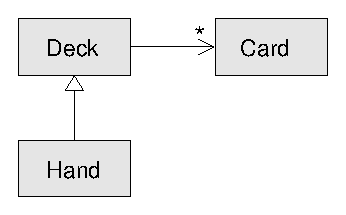
\includegraphics{figs/class1.eps}}
\afterfig

The arrow with a hollow triangle head represents an IS-A
relationship; in this case it indicates that Hand inherits
from Deck.

The standard arrow head represents a HAS-A
relationship; in this case a Deck has references to Card
objects.

\index{multiplicity (in class diagram)}

The star ({\tt *}) near the arrow head is a 
{\bf multiplicity}; it indicates how many Cards a Deck has.
A multiplicity can be a simple number, like {\tt 52}, a range,
like {\tt 5..7} or a star, which indicates that a Deck can
have any number of Cards.

A more detailed diagram might show that a Deck actually
contains a {\em list} of Cards, but built-in types
like list and dict are usually not included in class diagrams.

\begin{ex}
Read {\tt TurtleWorld.py}, {\tt World.py} and {\tt Gui.py}
and draw a class diagram that shows the relationships among
the classes defined there.
\end{ex}


\section{Debugging}
\index{debugging}

Inheritance can make debugging a challenge because when you
invoke a method on an object, you might not know which method
will be invoked.

\index{polymorphism}

Suppose you are writing a function that works with Hand objects.
You would like it to work with all kinds of Hands, like
PokerHands, BridgeHands, etc.  If you invoke a method like
{\tt shuffle}, you might get the one defined in {\tt Deck},
but if any of the subclasses override this method, you'll
get that version instead.  

\index{flow of execution}

Any time you are unsure about the flow of execution through your
program, the simplest solution is to add print statements at the
beginning of the relevant methods.  If {\tt Deck.shuffle} prints a
message that says something like {\tt Running Deck.shuffle}, then as
the program runs it traces the flow of execution.

As an alternative, you could use this function, which takes an
object and a method name (as a string) and returns the class that
provides the definition of the method:

\beforeverb
\begin{verbatim}
def find_defining_class(obj, meth_name):
    for ty in type(obj).mro():
        if meth_name in ty.__dict__:
            return ty
\end{verbatim}
\afterverb
%
Here's an example:

\beforeverb
\begin{verbatim}
>>> hand = Hand()
>>> print find_defining_class(hand, 'shuffle')
<class 'Card.Deck'>
\end{verbatim}
\afterverb
%
So the {\tt shuffle} method for this Hand is the one in {\tt Deck}.

\index{mro method}
\index{method!mro}
\index{method resolution order}

\verb"find_defining_class" uses the {\tt mro} method to get the list
of class objects (types) that will be searched for methods.  ``MRO''
stands for ``method resolution order.''

\index{override}
\index{interface}
\index{precondition}
\index{postcondition}

Here's a program design suggestion: whenever you override a method,
the interface of the new method should be the same as the old.  It
should take the same parameters, return the same type, and obey the
same preconditions and postconditions.  If you obey this rule, you
will find that any function designed to work with an instance of a
superclass, like a Deck, will also work with instances of subclasses
like a Hand or PokerHand.

If you violate this rule, your code will collapse like (sorry)
a house of cards.


\section{Glossary}

\begin{description}

\item[encode:]  To represent one set of values using another
set of values by constructing a mapping between them.
\index{encode}

\item[class attribute:] An attribute associated with a class
object.  Class attributes are defined inside
a class definition but outside any method.
\index{class attribute}
\index{attribute!class}

\item[instance attribute:] An attribute associated with an
instance of a class.
\index{instance attribute}
\index{attribute!instance}

\item[veneer:] A method or function that provides a different
interface to another function without doing much computation.
\index{veneer}

\item[inheritance:] The ability to define a new class that is a
modified version of a previously defined class.
\index{inheritance}

\item[parent class:] The class from which a child class inherits.
\index{parent class}

\item[child class:] A new class created by inheriting from an
existing class; also called a ``subclass.''
\index{child class}
\index{class!child}

\item[IS-A relationship:] The relationship between a child class
and its parent class.
\index{IS-A relationship}

\item[HAS-A relationship:] The relationship between two classes
where instances of one class contain references to instances of
the other.
\index{HAS-A relationship}

\item[class diagram:] A diagram that shows the classes in a program
and the relationships between them.
\index{class diagram}
\index{diagram!class}

\item[multiplicity:] A notation in a class diagram that shows, for
a HAS-A relationship, how many references there are to instances
of another class.
\index{multiplicity (in class diagram)}

\end{description}


\section{Exercises}

\begin{ex}
\index{poker}


The following are the possible hands in poker, in increasing order
of value (and decreasing order of probability):

\begin{description}

\item[pair:] two cards with the same rank
\vspace{-0.05in}

\item[two pair:] two pairs of cards with the same rank
\vspace{-0.05in}

\item[three of a kind:] three cards with the same rank
\vspace{-0.05in}

\item[straight:] five cards with ranks in sequence (aces can
be high or low, so {\tt Ace-2-3-4-5} is a straight and so is {\tt
10-Jack-Queen-King-Ace}, but {\tt Queen-King-Ace-2-3} is not.)
\vspace{-0.05in}

\item[flush:] five cards with the same suit
\vspace{-0.05in}

\item[full house:] three cards with one rank, two cards with another
\vspace{-0.05in}

\item[four of a kind:] four cards with the same rank
\vspace{-0.05in}

\item[straight flush:] five cards in sequence (as defined above) and
with the same suit
\vspace{-0.05in}

\end{description}
%
The goal of these exercises is to estimate
the probability of drawing these various hands.

\begin{enumerate}

\item Download the following files from \url{thinkpython.com/code}:

\begin{description}

\item[{\tt Card.py}]: A complete version of the {\tt Card},
{\tt Deck} and {\tt Hand} classes in this chapter.

\item[{\tt PokerHand.py}]: An incomplete implementation of a class
that represents a poker hand, and some code that tests it.

\end{description}
%
\item If you run {\tt PokerHand.py}, it deals seven 7-card poker hands
and checks to see if any of them contains a flush.  Read this
code carefully before you go on.

\item Add methods to {\tt PokerHand.py} named \verb"has_pair",
\verb"has_twopair", etc. that return True or False according to
whether or not the hand meets the relevant criteria.  Your code should
work correctly for ``hands'' that contain any number of cards
(although 5 and 7 are the most common sizes).

\item Write a method named {\tt classify} that figures out
the highest-value classification for a hand and sets the
{\tt label} attribute accordingly.  For example, a 7-card hand
might contain a flush and a pair; it should be labeled ``flush''.

\item When you are convinced that your classification methods are
working, the next step is to estimate the probabilities of the various
hands.  Write a function in {\tt PokerHand.py} that shuffles a deck of
cards, divides it into hands, classifies the hands, and counts the
number of times various classifications appear.

\item Print a table of the classifications and their probabilities.
Run your program with larger and larger numbers of hands until the
output values converge to a reasonable degree of accuracy.  Compare
your results to the values at \url{wikipedia.org/wiki/Hand_rankings}.

\end{enumerate}
\end{ex}


\begin{ex}

\index{Swampy}
\index{TurtleWorld}

This exercise uses TurtleWorld from Chapter~\ref{turtlechap}.
You will write code that makes Turtles play tag.  If you
are not familiar with the rules of tag, see
\url{wikipedia.org/wiki/Tag_(game)}.

\begin{enumerate}

\item Download \url{thinkpython.com/code/Wobbler.py} and run it.  You
should see a TurtleWorld with three Turtles.  If you press the
{\sf Run} button, the Turtles wander at random.

\item Read the code and make sure you understand how it works.
The {\tt Wobbler} class inherits from {\tt Turtle}, which means
that the {\tt Turtle} methods {\tt lt}, {\tt rt}, {\tt fd}
and {\tt bk} work on Wobblers.

The {\tt step} method gets invoked by TurtleWorld.  It invokes 
{\tt steer}, which turns the Turtle in the desired direction,
{\tt wobble}, which makes a random turn in proportion to the Turtle's
clumsiness, and {\tt move}, which moves forward a few pixels,
depending on the Turtle's speed.

\index{Tagger}

\item Create a file named {\tt Tagger.py}.  Import everything from
  {\tt Wobbler}, then define a class named {\tt Tagger} that inherits
  from {\tt Wobbler}.  Call \verb"make_world" passing the {\tt
    Tagger} class object as an argument.

\item Add a {\tt steer} method to {\tt Tagger} to override the one in
  {\tt Wobbler}.  As a starting place, write a version that always
  points the Turtle toward the origin.  Hint: use the math function
  {\tt atan2} and the Turtle attributes {\tt x}, {\tt y} and
  {\tt heading}.

\item Modify {\tt steer} so that the Turtles stay in bounds.
  For debugging, you might want to use the {\sf Step} button,
  which invokes {\tt step} once on each Turtle.

\item Modify {\tt steer} so that each Turtle points toward its nearest
  neighbor.  Hint: Turtles have an attribute, {\tt world}, that is a
  reference to the TurtleWorld they live in, and the TurtleWorld has
  an attribute, {\tt animals}, that is a list of all Turtles in the
  world.

\item Modify {\tt steer} so the Turtles play tag.  You can add methods
  to {\tt Tagger} and you can override {\tt steer} and
  \verb"__init__", but you may not modify or override {\tt step}, {\tt
    wobble} or {\tt move}.  Also, {\tt steer} is allowed to change the
  heading of the Turtle but not the position.

Adjust the rules and your {\tt steer} method for good quality play;
for example, it should be possible for the slow Turtle to tag the
faster Turtles eventually.

\end{enumerate}

You can get my solution from \url{thinkpython.com/code/Tagger.py}.
\end{ex}


\chapter{Case study: interface design}
\label{turtlechap}

\section{TurtleWorld}
\index{TurtleWorld}
\index{Swampy}

To accompany this book, I have written a suite of modules called
Swampy.  One of these modules is TurtleWorld, which provides
a set of functions for drawing lines by steering
turtles around the screen.

You can download Swampy from \url{thinkpython.com/swampy};
follow the instructions there to install Swampy on your system.

Move into the directory that contains {\tt TurtleWorld.py},
create a file named {\tt polygon.py} and type in the following
code:

\beforeverb
\begin{verbatim}
from TurtleWorld import *

world = TurtleWorld()
bob = Turtle()
print bob

wait_for_user()
\end{verbatim}
\afterverb
%
The first line is a variation of the {\tt import} statement we saw before;
instead of creating a module object, it imports the functions
from the module directly, so you can access them without using dot
notation.

\index{import statement}
\index{statement!import}

The next lines create a TurtleWorld assigned to {\tt world} and
a Turtle assigned to {\tt bob}.  Printing {\tt bob} yields something
like:

\beforeverb
\begin{verbatim}
<TurtleWorld.Turtle instance at 0xb7bfbf4c>
\end{verbatim}
\afterverb
%
This means that {\tt bob} refers to
an {\bf instance} of a Turtle
as defined in module {\tt TurtleWorld}.  In this context,
``instance'' means a member of a set;
this Turtle is one of the set of possible Turtles.

\index{instance}

\verb"wait_for_user" tells TurtleWorld to wait for the user
to do something, although in this case there's not much for
the user to do except close the window.

TurtleWorld provides several
turtle-steering functions: {\tt fd} and {\tt bk} for
forward and backward, and {\tt lt} and {\tt rt} for left and
right turns.  Also, each Turtle is holding a pen, which is
either down or up; if the pen is down, the Turtle leaves
a trail when it moves.  The functions {\tt pu} and {\tt pd}
stand for ``pen up'' and ``pen down.''

To draw a right angle, add these lines to the program
(after creating {\tt bob} and before calling \verb"wait_for_user"):

\beforeverb
\begin{verbatim}
fd(bob, 100)
rt(bob)
fd(bob, 100)
\end{verbatim}
\afterverb
%
The first line tells {\tt bob} to take 100 steps
forward.  The second line tells him to turn right.

When you run this program, you should see {\tt bob} move east and then
south, leaving two line segments behind.

Now modify the program to draw a square.  Don't go on until
you've got it working!

%\newpage

\section{Simple repetition}
\label{repetition}
\index{repetition}

Chances are you wrote something like this (leaving out the code
that creates TurtleWorld and waits for the user):

\begin{verbatim}
fd(bob, 100)
lt(bob)

fd(bob, 100)
lt(bob)

fd(bob, 100)
lt(bob)

fd(bob, 100)
\end{verbatim}
%
We can do the same thing more concisely with a {\tt for} statement.
Add this example to {\tt polygon.py} and run it again:

\index{for loop}
\index{loop!for}
\index{statement!for}

\beforeverb
\begin{verbatim}
for i in range(4):
    print 'Hello!'
\end{verbatim}
\afterverb
%
You should see something like this:

\beforeverb
\begin{verbatim}
Hello!
Hello!
Hello!
Hello!
\end{verbatim}
\afterverb
%
This is the simplest use of the {\tt for} statement; we will see
more later.  But that should be enough to let you rewrite your
square-drawing program.  Don't go on until you do.

%\newpage

Here is a {\tt for} statement that draws a square:

\beforeverb
\begin{verbatim}
for i in range(4):
    fd(bob, 100)
    lt(bob)
\end{verbatim}
\afterverb
%
The syntax of a {\tt for} statement is similar to a function
definition.  It has a header that ends with a colon and an indented
body.  The body can contain any number of statements.

\index{loop}

A {\tt for} statement is sometimes called a {\bf loop} because
the flow of execution runs through the body and then loops back
to the top.  In this case, it runs the body four times.

This version is actually a little different from the previous
square-drawing code because it makes another left turn after
drawing the last side of the square.  The extra turn takes a little
more time, but it simplifies the code if we do the same thing
every time through the loop.  This version also has the effect
of leaving the turtle back in the starting position, facing in
the starting direction.

\section{Exercises}

The following is a series of exercises using TurtleWorld.  They
are meant to be fun, but they have a point, too.  While you are
working on them, think about what the point is.

The following sections have solutions to the exercises, so
don't look until you have finished (or at least tried).

\begin{enumerate}

\item Write a function called {\tt square} that takes a parameter
named {\tt t}, which is a turtle.  It should use the turtle to draw
a square.

Write a function call that passes {\tt bob} as an argument to
{\tt square}, and then run the program again.

\item Add another parameter, named {\tt length}, to {\tt square}.
Modify the body so length of the sides is {\tt length}, and then
modify the function call to provide a second argument.  Run the
program again.  Test your program with a range of values for {\tt
length}.

\item The functions {\tt lt} and {\tt rt} make 90-degree turns by
default, but you can provide a second argument that specifies the
number of degrees.  For example, {\tt lt(bob, 45)} turns {\tt bob} 45
degrees to the left.

Make a copy of {\tt square} and change the name to {\tt polygon}.  Add
another parameter named {\tt n} and modify the body so it draws an
n-sided regular polygon.  Hint: The exterior angles of an n-sided regular
polygon are $360.0 / n$ degrees.

\index{polygon function}
\index{function!polygon}

\item Write a function called {\tt circle} that takes a turtle, {\tt t},
and radius, {\tt r}, as parameters and that draws an approximate circle
by invoking {\tt polygon} with an appropriate length and number of
sides.  Test your function with a range of values of {\tt r}.

\index{circle function}
\index{function!circle}

Hint: figure out the circumference of the circle and make sure that
{\tt length * n = circumference}.

Another hint: if {\tt bob} is too slow for you, you can speed
him up by changing {\tt bob.delay}, which is the time between moves,
in seconds.  {\tt bob.delay = 0.01} ought to get him moving.

\item Make a more general version of {\tt circle} called {\tt arc}
that takes an additional parameter {\tt angle}, which determines
what fraction of a circle to draw.  {\tt angle} is in units of
degrees, so when {\tt angle=360}, {\tt arc} should draw a complete
circle.

\index{arc function}
\index{function!arc}

\end{enumerate}

\section{Encapsulation}

The first exercise asks you to put your square-drawing code
into a function definition and then call the function, passing
the turtle as a parameter.  Here is a solution:

\beforeverb
\begin{verbatim}
def square(t):
    for i in range(4):
        fd(t, 100)
        lt(t)

square(bob)
\end{verbatim}
\afterverb
%
The innermost statements, {\tt fd} and {\tt lt} are
indented twice to show that they are inside the {\tt for} loop,
which is inside the function definition.  The next line,
{\tt square(bob)}, is flush with the left margin, so that is the
end of both the {\tt for} loop and the function definition.

Inside the function, {\tt t} refers to the same turtle {\tt bob}
refers to, so {\tt lt(t)} has the same effect as {\tt lt(bob)}.
So why not call the parameter {\tt bob}?  The idea is that {\tt t}
can be any turtle, not just {\tt bob}, so you could create
a second turtle and pass it as an argument to {\tt square}:

\beforeverb
\begin{verbatim}
ray = Turtle()
square(ray)
\end{verbatim}
\afterverb
%
Wrapping a piece of code up in a function is called {\bf
encapsulation}.  One of the benefits of encapsulation is that it
attaches a name to the code, which serves as a kind of documentation.
Another advantage is that if you re-use the code, it is more concise
to call a function twice than to copy and paste the body!

\index{encapsulation}


\section{Generalization}

The next step is to add a {\tt length} parameter to {\tt square}.
Here is a solution:

\beforeverb
\begin{verbatim}
def square(t, length):
    for i in range(4):
        fd(t, length)
        lt(t)

square(bob, 100)
\end{verbatim}
\afterverb
%
Adding a parameter to a function is called {\bf generalization}
because it makes the function more general: in the previous
version, the square is always the same size; in this version
it can be any size.

\index{generalization}

The next step is also a generalization.  Instead of drawing
squares, {\tt polygon} draws regular polygons with any number of
sides.  Here is a solution:

\beforeverb
\begin{verbatim}
def polygon(t, n, length):
    angle = 360.0 / n
    for i in range(n):
        fd(t, length)
        lt(t, angle)

polygon(bob, 7, 70)
\end{verbatim}
\afterverb
%
This draws a 7-sided polygon with side length 70.  If you have
more than a few numeric arguments, it is easy to forget what they
are, or what order they should be in.  It is legal, and sometimes
helpful, to include the names of the parameters in the argument
list:

\beforeverb
\begin{verbatim}
polygon(bob, n=7, length=70)
\end{verbatim}
\afterverb
%
These are called {\bf keyword arguments} because they include
the parameter names as ``keywords'' (not to be confused with
Python keywords like {\tt while} and {\tt def}).

\index{keyword argument}
\index{argument!keyword}

This syntax makes the program more readable.  It is also a reminder
about how arguments and parameters work: when you call a function, the
arguments are assigned to the parameters.


\section{Interface design}

The next step is to write {\tt circle}, which takes a radius,
{\tt r}, as a parameter.  Here is a simple solution that uses
{\tt polygon} to draw a 50-sided polygon:

\beforeverb
\begin{verbatim}
def circle(t, r):
    circumference = 2 * math.pi * r
    n = 50
    length = circumference / n
    polygon(t, n, length)
\end{verbatim}
\afterverb
%
The first line computes the circumference of a circle with radius
{\tt r} using the formula $2 \pi r$.  Since we use {\tt math.pi}, we
have to import {\tt math}.  By convention, {\tt import} statements
are usually at the beginning of the script.

{\tt n} is the number of line segments in our approximation of a circle,
so {\tt length} is the length of each segment.  Thus, {\tt polygon}
draws a 50-sides polygon that approximates a circle with radius {\tt r}.

One limitation of this solution is that {\tt n} is a constant, which
means that for very big circles, the line segments are too long, and
for small circles, we waste time drawing very small segments.  One
solution would be to generalize the function by taking {\tt n} as
a parameter.  This would give the user (whoever calls {\tt circle})
more control, but the interface would be less clean.

\index{interface}

The {\bf interface} of a function is a summary of how it is used: what
are the parameters?  What does the function do?  And what is the return
value?  An interface is ``clean'' if it is ``as simple as
possible, but not simpler. (Einstein)''

\index{Einstein, Albert}

In this example, {\tt r} belongs in the interface because it
specifies the circle to be drawn.  {\tt n} is less appropriate
because it pertains to the details of {\em how} the circle should
be rendered.

Rather than clutter up the interface, it is better
to choose an appropriate value of {\tt n}
depending on {\tt circumference}:

\beforeverb
\begin{verbatim}
def circle(t, r):
    circumference = 2 * math.pi * r
    n = int(circumference / 3) + 1
    length = circumference / n
    polygon(t, n, length)
\end{verbatim}
\afterverb
%
Now the number of segments is (approximately) {\tt circumference/3},
so the length of each segment is (approximately) 3, which is small
enough that the circles look good, but big enough to be efficient,
and appropriate for any size circle.


\section{Refactoring}
\label{refactoring}
\index{refactoring}

When I wrote {\tt circle}, I was able to re-use {\tt polygon}
because a many-sided polygon is a good approximation of a circle.
But {\tt arc} is not as cooperative; we can't use {\tt polygon}
or {\tt circle} to draw an arc.

One alternative is to start with a copy
of {\tt polygon} and transform it into {\tt arc}.  The result
might look like this:

\beforeverb
\begin{verbatim}
def arc(t, r, angle):
    arc_length = 2 * math.pi * r * angle / 360
    n = int(arc_length / 3) + 1
    step_length = arc_length / n
    step_angle = float(angle) / n
    
    for i in range(n):
        fd(t, step_length)
        lt(t, step_angle)
\end{verbatim}
\afterverb
%
The second half of this function looks like {\tt polygon}, but we
can't re-use {\tt polygon} without changing the interface.  We could
generalize {\tt polygon} to take an angle as a third argument,
but then {\tt polygon} would no longer be an appropriate name!
Instead, let's call the more general function {\tt polyline}:

\beforeverb
\begin{verbatim}
def polyline(t, n, length, angle):
    for i in range(n):
        fd(t, length)
        lt(t, angle)
\end{verbatim}
\afterverb
%
Now we can rewrite {\tt polygon} and {\tt arc} to use {\tt polyline}:

\beforeverb
\begin{verbatim}
def polygon(t, n, length):
    angle = 360.0 / n
    polyline(t, n, length, angle)

def arc(t, r, angle):
    arc_length = 2 * math.pi * r * angle / 360
    n = int(arc_length / 3) + 1
    step_length = arc_length / n
    step_angle = float(angle) / n
    polyline(t, n, step_length, step_angle)
\end{verbatim}
\afterverb
%
Finally, we can rewrite {\tt circle} to use {\tt arc}:

\beforeverb
\begin{verbatim}
def circle(t, r):
    arc(t, r, 360)
\end{verbatim}
\afterverb
%
This process---rearranging a program to improve function
interfaces and facilitate code re-use---is called {\bf refactoring}.
In this case, we noticed that there was similar code in {\tt arc} and
{\tt polygon}, so we ``factored it out'' into {\tt polyline}.

\index{refactoring}

If we had planned ahead, we might have written {\tt polyline} first
and avoided refactoring, but often you don't know enough at the
beginning of a project to design all the interfaces.  Once you start
coding, you understand the problem better.  Sometimes refactoring is a
sign that you have learned something.


\section{A development plan}
\index{development plan!encapsulation and generalization}

A {\bf development plan} is a process for writing programs.
The process we used
in this case study is ``encapsulation and
generalization.''  The steps of this process are:

\begin{enumerate}

\item Start by writing a small program with no function definitions.

\item Once you get the program working, encapsulate it in a function
and give it a name.

\item Generalize the function by adding appropriate parameters.

\item Repeat steps 1--3 until you have a set of working functions.
Copy and paste working code to avoid retyping (and re-debugging).

\item Look for opportunities to improve the program by refactoring.
For example, if you have similar code in several places, consider
factoring it into an appropriately general function.

\end{enumerate}

This process has some drawbacks---we will see alternatives later---but
it can be useful if you don't know ahead of time how to divide the
program into functions.  This approach lets you design as you go
along.


\section{docstring}
\label{docstring}
\index{docstring}

A {\bf docstring} is a string at the beginning of a function that
explains the interface (``doc'' is short for ``documentation'').  Here
is an example:

\beforeverb
\begin{verbatim}
def polyline(t, length, n, angle):
    """Draw n line segments with the given length and
    angle (in degrees) between them.  t is a turtle.
    """    
    for i in range(n):
        fd(t, length)
        lt(t, angle)
\end{verbatim}
\afterverb
%
This docstring is a triple-quoted string, also known
as a multiline string because the triple quotes allow the string
to span more than one line.

\index{quotation mark}
\index{triple-quoted string}
\index{string!triple-quoted}
\index{multiline string}
\index{string!multiline}

It is terse, but it contains the essential information
someone would need to use this function.  It explains concisely what
the function does (without getting into the details of how it does
it).  It explains what effect each parameter has on the behavior of
the function and what type each parameter should be (if it is not
obvious).

Writing this kind of documentation is an important part of interface
design.  A well-designed interface should be simple to explain;
if you are having a hard time explaining one of your functions,
that might be a sign that the interface could be improved.


\section{Debugging}
\index{debugging}
\index{interface}

An interface is like a contract between a function and a caller.
The caller agrees to provide certain parameters and the function
agrees to do certain work.

For example, {\tt polyline} requires four arguments.  The first
has to be a Turtle (or some other object that works with {\tt fd}
and {\tt lt}).  The second has to be a number, and it should
probably be positive, although it turns out that the function
works even if it isn't.  The third argument should be an integer;
{\tt range} complains otherwise (depending on which version
of Python you are running).  The fourth has to be a number,
which is understood to be in degrees.

These requirements are called {\bf preconditions} because they
are supposed to be true before the function starts executing.
Conversely, conditions at the end of the function are
{\bf postconditions}.  Postconditions include the intended
effect of the function (like drawing line segments) and any
side effects (like moving the Turtle or making other changes
in the World).

\index{precondition}
\index{postcondition}

Preconditions are the responsibility of the caller.  If the caller
violates a (properly documented!) precondition and the function
doesn't work correctly, the bug is in the caller, not the function.
However, for purposes of debugging it is often a good idea for
functions to check their preconditions rather than assume they are
true.  If every function checks its preconditions before starting,
then if something goes wrong, you will know which function to blame.


\section{Glossary}

\begin{description}

\item[instance:] A member of a set.  The TurtleWorld in this
chapter is a member of the set of TurtleWorlds.
\index{instance}

\item[loop:] A part of a program that can execute repeatedly.
\index{loop}

\item[encapsulation:] The process of transforming a sequence of
statements into a function definition.
\index{encapsulation}

\item[generalization:] The process of replacing something
unnecessarily specific (like a number) with something appropriately
general (like a variable or parameter).
\index{generalization}

\item[keyword argument:] An argument that includes the name of
the parameter as a ``keyword.''
\index{keyword argument}
\index{argument!keyword}

\item[interface:] A description of how to use a function, including
the name and descriptions of the arguments and return value.
\index{interface}

\item[development plan:] A process for writing programs.
\index{development plan}

\item[docstring:]  A string that appears in a function definition
to document the function's interface.
\index{docstring}

\item[precondition:] A requirement that should be satisfied by
the caller before a function starts.
\index{precondition}

\item[postcondition:] A requirement that should be satisfied by
the function before it ends.
\index{precondition}

\end{description}


\section{Exercises}

\begin{ex}

Download the code in this chapter from
\url{thinkpython.com/code/polygon.py}.

\begin{enumerate}

\item Write appropriate docstrings for {\tt polygon}, {\tt arc} and
{\tt circle}.

\index{stack diagram}

\item Draw a stack diagram that shows the state of the program
while executing {\tt circle(bob, radius)}.  You can do the
arithmetic by hand or add {\tt print} statements to the code.


\item The version of {\tt arc} in Section~\ref{refactoring} is not
very accurate because the linear approximation of the
circle is always outside the true circle.  As a result,
the turtle ends up a few units away from the correct
destination. My solution shows a way to reduce
the effect of this error.  Read the code and see if it makes
sense to you.  If you draw a diagram, you might see how it works.

\end{enumerate}

\end{ex}


\begin{ex}
\index{flower}

Write an appropriately general set of functions that
can draw flowers like this:

\centerline{
\includegraphics[height=1in]{figs/flowers.eps}}

You can download a solution from \url{thinkpython.com/code/flower.py}.

\end{ex}


\begin{ex}
\index{pie}

Write an appropriately general set of functions that
can draw shapes like this:

\centerline{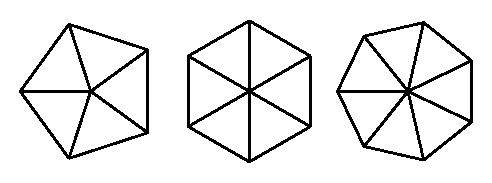
\includegraphics[height=0.9in]{figs/pies.eps}}

You can download a solution from \url{thinkpython.com/code/pie.py}.

\end{ex}

\begin{ex}
\index{alphabet}
\index{turtle typewriter}
\index{typewriter, turtle}

The letters of the alphabet can be constructed from a moderate
number of basic elements, like vertical and horizontal lines
and a few curves.  Design a font that can be drawn with a
minimal number of basic elements and then write functions
that draw letters of the alphabet.

You should write one function for each letter, with names
\verb"draw_a", \verb"draw_b", etc., and put your functions
in a file named {\tt letters.py}.  You can download a
``turtle typewriter'' from \url{thinkpython.com/code/typewriter.py}
to help you test your code.

You can download a solution from \url{thinkpython.com/code/letters.py}.

\end{ex}




\chapter{Case study: Tkinter}

\section{GUI}

Most of the programs we have seen so far are text-based, but
many programs use {\bf graphical user interfaces}, also
known as {\bf GUIs}.

\index{GUI}
\index{graphical user interface}
\index{Tkinter}

Python provides several choices for writing GUI-based programs,
including wxPython, Tkinter, and Qt.  Each has pros and cons, which
is why Python has not converged on a standard.

The one I will present in this chapter is Tkinter because I think
it is the easiest to get started with.  Most of the concepts
in this chapter apply to the other GUI modules, too.

There are several books and web pages about Tkinter.  One of
the best online resources is {\em An Introduction to Tkinter}
by Fredrik Lundh.

\index{Gui module}
\index{module!Gui}
\index{Swampy}

I have written a module called {\tt Gui.py} that comes with
Swampy.  It provides a simplified interface to the functions
and classes in Tkinter.  The examples in this chapter are
based on this module.

Here is a simple example that creates and displays a Gui:

To create a GUI, you have to import {\tt Gui} and instantiate
a Gui object:

\beforeverb
\begin{verbatim}
from Gui import *

g = Gui()
g.title('Gui')
g.mainloop()
\end{verbatim}
\afterverb
%
When you run this code, a window should appear with an empty gray
square and the title {\sf Gui}.  {\tt mainloop} runs the {\bf event
  loop}, which waits for the user to do something and responds
accordingly.  It is an infinite loop; it runs until the user closes
the window, or presses Control-C, or does something that causes the
program to quit.

\index{event loop}
\index{loop!event}
\index{infinite loop}
\index{loop!infinite}

This Gui doesn't do much because it doesn't have any
{\bf widgets}.  Widgets are the elements that make up a
GUI; they include:

\index{widget}

\begin{description}

\item[Button:] A widget, containing text or an image, that
performs an action when pressed.

\item[Canvas:] A region that can display lines, rectangles,
circles and other shapes.

\item[Entry:] A region where users can type text.

\item[Scrollbar:] A widget that controls the visible part of another
widget.

\item[Frame:] A container, often invisible, that contains other
widgets.

\end{description}

The empty gray square you see when you create a Gui is
a Frame.  When you create a new widget, it is added to this Frame.



\section{Buttons and callbacks}

\index{Button widget}
\index{widget!Button}

The method {\tt bu} creates a Button widget:

\beforeverb
\begin{verbatim}
button = g.bu(text='Press me.')
\end{verbatim}
\afterverb
%
The return value from {\tt bu} is a Button object.  The button
that appears in the Frame is a graphical representation of this
object; you can control the button by invoking methods on it.

\index{option}

{\tt bu} takes up to 32 parameters that control the appearance
and function of the button.  These parameters are called
{\bf options}.  Instead of providing values for all 32 options,
you can use keyword arguments, like \verb"text='Press me.'",
to specify only the options you need and use the default
values for the rest.

\index{keyword argument}
\index{argument!keyword}

When you add a widget to the Frame, it gets ``shrink-wrapped;''
that is, the Frame shrinks to the size of the Button.  If you
add more widgets, the Frame grows to accommodate them.

\index{Label widget}
\index{widget!Label}

The method {\tt la} creates a Label widget:

\beforeverb
\begin{verbatim}
label = g.la(text='Press the button.')
\end{verbatim}
\afterverb
%
By default, Tkinter stacks the widgets top-to-bottom and centers
them.  We'll see how to override that behavior soon.

If you press the button, you will see that it doesn't do much.
That's because you haven't ``wired it up;'' that is, you haven't
told it what to do!

The option that controls the behavior of a button is {\tt command}.
The value of {\tt command} is a function that gets executed when
the button is pressed.  For example, here is a function that creates
a new Label:

\beforeverb
\begin{verbatim}
def make_label():
    g.la(text='Thank you.')
\end{verbatim}
\afterverb
%
Now we can create a button with this function as its command:

\beforeverb
\begin{verbatim}
button2 = g.bu(text='No, press me!', command=make_label)
\end{verbatim}
\afterverb
%
When you press this button, it should execute \verb"make_label"
and a new label should appear.

\index{callback}

The value of the {\tt command} option
is a function object, which is known as a {\bf callback} because
after you call {\tt bu} to create the button, the flow of execution
``calls back'' when the user presses the button.

\index{event-driven programming}

This kind of flow is characteristic of {\bf event-driven programming}.
User actions, like button presses and key strokes, are called {\bf
events}.  In event-driven programming, the flow of execution is
determined by user actions rather than by the programmer.  

The challenge of event-driven programming is to construct a set of
widgets and callbacks that work correctly (or at least generate
appropriate error messages) for any sequence of user actions.

\begin{ex}
Write a program that creates a GUI with a single button.  When the
button is pressed it should create a second button.  When
{\em that} button is pressed, it should create a label that
says, ``Nice job!''.

What happens if you press the buttons more than once?
You can see my solution at \url{thinkpython.com/code/button_demo.py}

\end{ex}


\section{Canvas widgets}

\index{Canvas widget}
\index{widget!Canvas}

One of the most versatile widgets is the Canvas, which creates
a region for drawing lines, circles and other shapes.  If you
did Exercise~\ref{canvas} you are already familiar with canvases.

The method {\tt ca} creates a new Canvas:

\beforeverb
\begin{verbatim}
canvas = g.ca(width=500, height=500)
\end{verbatim}
\afterverb
%
{\tt width} and {\tt height} are the dimensions of the canvas
in pixels.  

\index{config method}
\index{method!config}

After you create a widget, you can still change the values of
the options with the
{\tt config} method.  For example, the {\tt bg} option changes
the background color:

\beforeverb
\begin{verbatim}
canvas.config(bg='white')
\end{verbatim}
\afterverb
%
The value of {\tt bg} is a string
that names a color.  The set of legal color names is different
for different implementations of Python, but all implementations
provide at least:

\beforeverb
\begin{verbatim}
white   black
red     green    blue   
cyan    yellow   magenta
\end{verbatim}
\afterverb
%
Shapes on a Canvas are called {\bf items}.  For example,
the Canvas method {\tt circle} draws (you guessed it) a circle:

\index{Canvas item}
\index{item!Canvas}

\beforeverb
\begin{verbatim}
item = canvas.circle([0,0], 100, fill='red')
\end{verbatim}
\afterverb
%
The first argument is a coordinate pair that specifies the
center of the circle; the second is the radius.

\index{Canvas coordinate}
\index{coordinate!Canvas}

{\tt Gui.py} provides a standard Cartesian coordinate system with
the origin at the center of the Canvas and the positive $y$ axis
pointing up.  This is different from some other graphics systems
where the the origin is in the upper left with the $y$ axis
pointing down.

The {\tt fill} option specifies that the circle should be filled
in with red.

The return value from {\tt circle} is an Item object that
provides methods for modifying the item on the canvas.  For
example, you can use {\tt config} to change any of the circle's
options:

\beforeverb
\begin{verbatim}
item.config(fill='yellow', outline='orange', width=10)
\end{verbatim}
\afterverb
%
{\tt width} is the thickness of the outline in pixels;
{\tt outline} is the color.

\begin{ex}
\label{circle}
Write a program that creates a Canvas and a Button.  When the
user presses the Button, it should draw a circle on the canvas.
\end{ex}


\section{Coordinate sequences}

\index{coordinate sequence}
\index{sequence!coordinate}

The {\tt rectangle} method takes a sequence of coordinates that
specify opposite corners of the rectangle.  This example
draws a green rectangle with the lower left corner at the origin
and the upper right corner at $(200, 100)$:

\beforeverb
\begin{verbatim}
canvas.rectangle([[0, 0], [200, 100]], 
                 fill='blue', outline='orange', width=10)
\end{verbatim}
\afterverb
%
This way of specifying corners is called
a {\bf bounding box} because the two points
bound the rectangle.

\index{bounding box}

{\tt oval} takes a bounding box and draws an oval
within the specified rectangle:

\beforeverb
\begin{verbatim}
canvas.oval([[0, 0], [200, 100]], outline='orange', width=10)
\end{verbatim}
\afterverb
%
{\tt line} takes a sequence of coordinates and draws
a line that connects the points.  This example draws two legs
of a triangle:

\beforeverb
\begin{verbatim}
canvas.line([[0, 100], [100, 200], [200, 100]], width=10)
\end{verbatim}
\afterverb
%
{\tt polygon} takes the same arguments, but it draws the last
leg of the polygon (if necessary) and fills it in:

\beforeverb
\begin{verbatim}
canvas.polygon([[0, 100], [100, 200], [200, 100]],
               fill='red', outline='orange', width=10)
\end{verbatim}
\afterverb
%


\section{More widgets}

\index{Text widget}
\index{widget!Text}

Tkinter provides two widgets that let users type text: an
Entry, which is a single line, and a Text widget, which has
multiple lines.

\index{Entry widget}
\index{widget!Entry}

{\tt en} creates a new Entry:

\beforeverb
\begin{verbatim}
entry = g.en(text='Default text.')
\end{verbatim}
\afterverb
%
The {\tt text} option allows you to put text into the entry
when it is created.  The {\tt get} method returns the contents
of the Entry (which may have been changed by the user):

\beforeverb
\begin{verbatim}
>>> entry.get()
'Default text.'
\end{verbatim}
\afterverb
%
{\tt te} creates a Text widget:

\beforeverb
\begin{verbatim}
text = g.te(width=100, height=5)
\end{verbatim}
\afterverb
%
{\tt width} and {\tt height} are the dimensions of the
widget in characters and lines.

{\tt insert} puts text into the Text widget:

\beforeverb
\begin{verbatim}
text.insert(END, 'A line of text.')
\end{verbatim}
\afterverb
%
{\tt END} is a special index that indicates the last character in the
Text widget.

You can also specify a character using a dotted index, like {\tt 1.1},
which has the line number before the dot and the column number after.
The following example adds the letters \verb"'nother'" after the first
character of the first line.

\beforeverb
\begin{verbatim}
>>> text.insert(1.1, 'nother')
\end{verbatim}
\afterverb
%
The {\tt get} method reads the text in the widget; it takes a start
and end index as arguments.  The following example returns all the
text in the widget, including the newline character:

\beforeverb
\begin{verbatim}
>>> text.get(0.0, END)
'Another line of text.\n'
\end{verbatim}
\afterverb
%
The {\tt delete} method removes text from the widget;
the following example deletes all but the first two characters:

\beforeverb
\begin{verbatim}
>>> text.delete(1.2, END)
>>> text.get(0.0, END)
'An\n'
\end{verbatim}
\afterverb
%

\begin{ex}
\label{circle2}

Modify your solution to Exercise~\ref{circle} by adding an
Entry widget and a second button.  When the user presses the
second button, it should read a color name from the Entry and
use it to change the fill color of the circle.  Use {\tt config}
to modify the existing circle; don't create a new one.

Your program should handle the case where the user tries to
change the color of a circle that hasn't been created, and
the case where the color name is invalid.

You can see my solution at \url{thinkpython.com/code/circle_demo.py}.

\end{ex}


\section{Packing widgets}

So far we have been stacking widgets in a single column, but in most
GUIs the layout is more complicated.  For example, here is a slightly
simplified version of TurtleWorld (see
Chapter~\ref{turtlechap}).

\beforefig
\centerline{
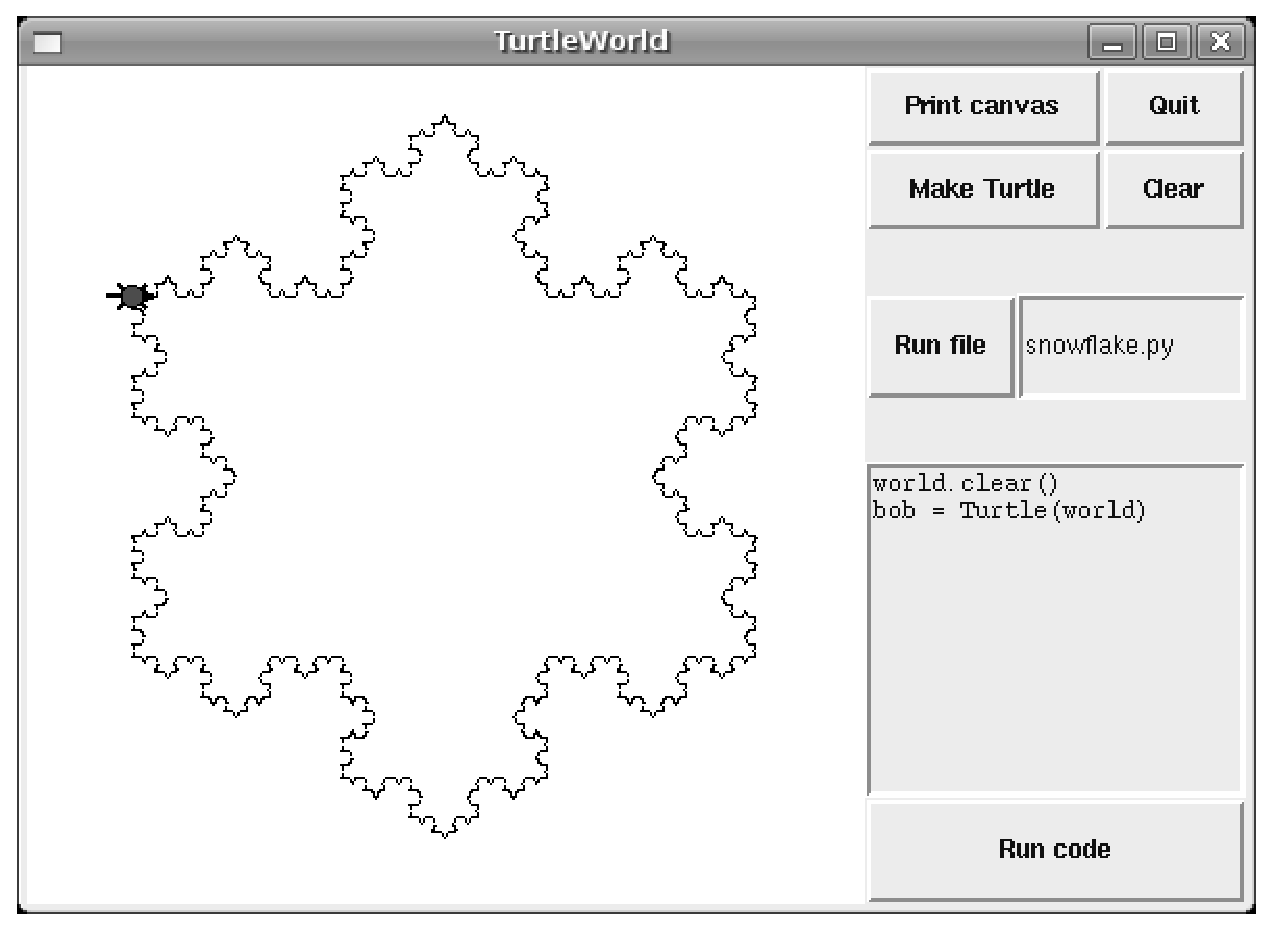
\includegraphics[width=1.0\textwidth]{figs/TurtleWorld.eps}
}
\afterfig

This section presents the code that creates this GUI, broken into a
series of steps.  You can download the complete example
from \url{thinkpython.com/code/SimpleTurtleWorld.py}.

At the top level, this GUI contains two widgets---a Canvas and a
Frame---arranged in a row.  So the first step is to create the row.

\index{SimpleTurtleWorld class}
\index{class!SimpleTurtleWorld}

\beforeverb
\begin{verbatim}
class SimpleTurtleWorld(TurtleWorld):
    """This class is identical to TurtleWorld, but the code that
    lays out the GUI is simplified for explanatory purposes."""

    def setup(self):
        self.row()
        ...
\end{verbatim}
\afterverb
%
{\tt setup} is the function that creates and arranges the widgets.
Arranging widgets in a GUI is called {\bf packing}.

\index{packing widgets}
\index{widget, packing}
\index{Frame widget}
\index{widget!Frame}

{\tt row} creates a row Frame and makes it the ``current Frame.''
Until this Frame is closed or another Frame is created, all
subsequent widgets are packed in a row.

Here is the code that creates the Canvas and the column Frame
that hold the other widgets:

\beforeverb
\begin{verbatim}
        self.canvas = self.ca(width=400, height=400, bg='white')
        self.col()
\end{verbatim}
\afterverb
%
The first widget in the column is a grid Frame, which contains
four buttons arranged two-by-two:

\beforeverb
\begin{verbatim}
        self.gr(cols=2)
        self.bu(text='Print canvas', command=self.canvas.dump)
        self.bu(text='Quit', command=self.quit)
        self.bu(text='Make Turtle', command=self.make_turtle)
        self.bu(text='Clear', command=self.clear)
        self.endgr()
\end{verbatim}
\afterverb
%
{\tt gr} creates the grid; the argument is the number of
columns.  Widgets in the grid are
layed out left-to-right, top-to-bottom.

\index{callback}
\index{bound method}
\index{method, bound}
\index{subject}

The first button uses {\tt self.canvas.dump} as a callback; the second
uses {\tt self.quit}.  These are {\bf bound methods}, which means they
are associated with a particular object.  When they are invoked, they
are invoked on the object.

The next widget in the column is a row Frame that contains
a Button and an Entry:

\beforeverb
\begin{verbatim}
        self.row([0,1], pady=30)
        self.bu(text='Run file', command=self.run_file)
        self.en_file = self.en(text='snowflake.py', width=5)
        self.endrow()
\end{verbatim}
\afterverb
%
The first argument to {\tt row} is a list of weights that
determines how extra space is allocated between widgets.  
The list {\tt [0,1]} means that all extra space is allocated
to the second widget, which is the Entry.  If you run this code
and resize the window, you will see that the Entry grows and
the Button doesn't.

The option {\tt pady} ``pads'' this row in the $y$ direction,
adding 30 pixels of space above and below.

{\tt endrow} ends this row of widgets, so subsequent widgets are
packed in the column Frame.  {\tt Gui.py} keeps a stack of Frames:

\begin{itemize}

\item When you use {\tt row}, {\tt col} or {\tt gr} to create a Frame,
it goes on top of the stack and becomes the current Frame.

\item When you use {\tt endrow}, {\tt endcol} or {\tt endgr} to close
a Frame, it gets popped off the stack and the previous Frame on the
stack becomes the current Frame.

\end{itemize} 

The method \verb"run_file" reads the contents of the Entry,
uses it as a filename, reads the contents
and passes it to \verb"run_code".  {\tt self.inter} is an
Interpreter object that knows how to take a string and
execute it as Python code.

\beforeverb
\begin{verbatim}
    def run_file(self):
        filename = self.en_file.get()
        fp = open(filename)
        source = fp.read()
        self.inter.run_code(source, filename)
\end{verbatim}
\afterverb
%
The last two widgets are a Text widget and a Button:

\beforeverb
\begin{verbatim}
        self.te_code = self.te(width=25, height=10)
        self.te_code.insert(END, 'world.clear()\n')
        self.te_code.insert(END, 'bob = Turtle(world)\n')

        self.bu(text='Run code', command=self.run_text)
\end{verbatim}
\afterverb
%
\verb"run_text" is similar to \verb"run_file" except that it takes
the code from the Text widget instead of from a file:

\beforeverb
\begin{verbatim}
    def run_text(self):
        source = self.te_code.get(1.0, END)
        self.inter.run_code(source, '<user-provided code>')
\end{verbatim}
\afterverb
%
Unfortunately, the details of widget layout are different in
other languages, and in different Python modules.
Tkinter alone provides three different mechanisms for arranging
widgets.  These mechanisms are called {\bf geometry managers}.
The one I demonstrated in this section is the ``grid'' geometry
manager; the others are called ``pack'' and ``place''.

\index{geometry manager}

Fortunately, most of the concepts in this section apply to
other GUI modules and other languages.


\section{Menus and Callables}

\index{Menubutton widget}
\index{widget!Menubutton}

A Menubutton is a widget that looks like a button, but when pressed
it pops up a menu.  After the user selects an item, the menu
disappears.

Here is code that creates a color selection Menubutton
(you can download it from \url{thinkpython.com/code/menubutton_demo.py}):

% mb_example.py

\beforeverb
\begin{verbatim}
g = Gui()
g.la('Select a color:')
colors = ['red', 'green', 'blue']
mb = g.mb(text=colors[0])
\end{verbatim}
\afterverb
%
{\tt mb} creates the Menubutton.  Initially, the text on the button is
the name of the default color.  The following loop creates one menu
item for each color:

\beforeverb
\begin{verbatim}
for color in colors:
    g.mi(mb, text=color, command=Callable(set_color, color))
\end{verbatim}
\afterverb
%
The first argument of {\tt mi} is the Menubutton these items are
associated with.

\index{callback}
\index{Callable object}
\index{object!Callable}

The {\tt command} option is a Callable object, which is something new.
So far we have seen functions and bound methods used as callbacks,
which works fine if you don't have to pass any arguments to
the function.  Otherwise you have to construct a Callable object
that contains a function, like \verb"set_color", and its arguments,
like {\tt color}.

The Callable object stores a reference to the function and the
arguments as attributes.  Later, when the user clicks on a menu
item, the callback calls the function and passes the stored
arguments.

Here is what \verb"set_color" might look like:

\beforeverb
\begin{verbatim}
def set_color(color):
    mb.config(text=color)
    print color
\end{verbatim}
\afterverb
%
When the user selects a menu item and \verb"set_color" is called,
it configures the Menubutton to display the newly-selected color.
It also print the color; if you try this example, you can confirm that
\verb"set_color" is called when you select an item (and {\em not}
called when you create the Callable object).


\section{Binding}

\index{binding}
\index{callback}

A {\bf binding} is an association between a widget, an event and a
callback: when an event (like a button press) happens on a widget, the
callback is invoked.

Many widgets have default bindings.  For example, when you press
a button, the default binding changes the relief of the button
to make it look depressed.  When you release the button, the
binding restores the appearance of the button and invokes the
callback specified with the {\tt command} option.

You can use the {\tt bind} method to override these default
bindings or to add new ones.  For example, this code creates a
binding for a canvas (you can download the code in this
section from \url{thinkpython.com/code/draggable_demo.py}):

\beforeverb
\begin{verbatim}
ca.bind('<ButtonPress-1>', make_circle)
\end{verbatim}
\afterverb
%
The first argument is an event string; this event is triggered
when the user presses the left mouse button.  Other mouse
events include {\tt ButtonMotion}, {\tt ButtonRelease} and
{\tt Double-Button}.

\index{event string}
\index{event handler}

The second argument is an event handler.  An event handler
is a function or bound method, like a callback, but an important
difference is that an event handler takes an Event object as a
parameter.  Here is an example:

\beforeverb
\begin{verbatim}
def make_circle(event):
    pos = ca.canvas_coords([event.x, event.y])
    item = ca.circle(pos, 5, fill='red')
\end{verbatim}
\afterverb
%
The Event object contains information about the type of event and
details like the coordinates of the mouse pointer.  In this example
the information we need is
the location of the mouse click.  These
values are in ``pixel coordinates,'' which are defined by the
underlying graphical system.  The method \verb"canvas_coords"
translates them to ``Canvas coordinates,'' which are compatible with
Canvas methods like {\tt circle}.

\index{Event object}
\index{object!Event}

For Entry widgets, it is common to bind the \verb"<Return>" event,
which is triggered when the user presses the {\sf Return} or
{\sf Enter} key.  For example, the following code creates a Button
and an Entry.

\beforeverb
\begin{verbatim}
bu = g.bu('Make text item:', make_text)
en = g.en()
en.bind('<Return>', make_text)
\end{verbatim}
\afterverb
%
\verb"make_text" is called when the Button is pressed or when
the user hits {\sf Return} while typing in the Entry.  To make
this work, we need a function that can be called as a command
(with no arguments) or as an event handler (with an Event
as an argument):

\beforeverb
\begin{verbatim}
def make_text(event=None):
    text = en.get()
    item = ca.text([0,0], text)
\end{verbatim}
\afterverb
%
\verb"make_text" gets the contents of the Entry and displays
it as a Text item in the Canvas.

It is also possible to create bindings for Canvas items.
The following is a class definition for {\tt Draggable},
which is a child class of {\tt Item} that provides bindings
that implement drag-and-drop capability.

\index{drag-and-drop}

\beforeverb
\begin{verbatim}
class Draggable(Item):

    def __init__(self, item):
        self.canvas = item.canvas
        self.tag = item.tag
        self.bind('<Button-3>', self.select)
        self.bind('<B3-Motion>', self.drag)
        self.bind('<Release-3>', self.drop)
\end{verbatim}
\afterverb
%
The init method takes an Item as a parameter.  It copies
the attributes of the Item and then creates bindings for
three events: a button press, button motion, and button release.

The event handler {\tt select} stores the coordinates
of the current event and the original color of the item, then
changes the color to yellow:

\beforeverb
\begin{verbatim}
    def select(self, event):
        self.dragx = event.x
        self.dragy = event.y

        self.fill = self.cget('fill')
        self.config(fill='yellow')
\end{verbatim}
\afterverb
%
{\tt cget} stands for ``get configuration;'' it takes the name of an
option as a string and returns the current value of that option.

{\tt drag} computes how far the object has moved relative to the
starting place, updates the stored coordinates, and then moves the
item.

\index{update!coordinate}

\beforeverb
\begin{verbatim}
    def drag(self, event):
        dx = event.x - self.dragx
        dy = event.y - self.dragy

        self.dragx = event.x
        self.dragy = event.y

        self.move(dx, dy)
\end{verbatim}
\afterverb
%
This computation is done in pixel coordinates; there is no need to
convert to Canvas coordinates.

\index{Canvas coordinate}
\index{coordinate!Canvas}
\index{pixel coordinate}
\index{coordinate!pixel}

Finally, {\tt drop} restores the original color of the item:

\beforeverb
\begin{verbatim}
    def drop(self, event):
        self.config(fill=self.fill)
\end{verbatim}
\afterverb
%
You can use the {\tt Draggable} class to add drag-and-drop
capability to an existing item.  For example, here is a modified
version of \verb"make_circle" that uses {\tt circle} to create
an Item and {\tt Draggable} to make it draggable:

\beforeverb
\begin{verbatim}
def make_circle(event):
    pos = ca.canvas_coords([event.x, event.y])
    item = ca.circle(pos, 5, fill='red')
    item = Draggable(item)
\end{verbatim}
\afterverb
%
This example demonstrates one of the benefits of inheritance: you can
modify the capabilities of a parent class without modifying its
definition.  This is particularly useful if you want to change
behavior defined in a module you did not write.


\section{Debugging}
\index{debugging}

One of the challenges of GUI programming is keeping track of
which things happen while the GUI is being built and which
things happen later in response to user events.

\index{callback}

For example, when you are setting up a callback, it is a common error
to call the function rather than passing a reference to it:

\beforeverb
\begin{verbatim}
def the_callback():
    print 'Called.'

g.bu(text='This is wrong!', command=the_callback())
\end{verbatim}
\afterverb
%
If you run this code, you will see that it calls \verb"the_callback"
immediately, and {\em then} creates the button.  When you press the
button, it does nothing because the return value from 
\verb"the_callback" is {\tt None}.
Usually you do not want to invoke a callback while you are
setting up the GUI; it should only be invoked later in response to
a user event.

\index{flow of execution}
\index{event-driven programming}

Another challenge of GUI programming is that you don't have control
of the flow of execution.  Which parts of the program execute
and their order are determined by user actions.
That means that you have to design your program to work correctly
for any possible sequence of events.

For example, the GUI in Exercise~\ref{circle2} has two widgets:
one creates a Circle item and the other changes the color of the
Circle.  If the user creates the circle and then changes its color,
there's no problem.  But what if the user changes the color of
a circle that doesn't exist yet?  Or creates more than one circle?

As the number of widgets grows, it is increasingly difficult to
imagine all possible sequences of events.  One way to manage this 
complexity is to encapsulate the state of the system in an object
and then consider:

\begin{itemize}

\item What are the possible states?  In the Circle example, we
might consider two states: before and after the user creates the
first circle.

\item In each state, what events can occur?  In the example,
the user can press either of the buttons, or quit.

\item For each state-event pair, what is the desired outcome?
Since there are two states and two buttons, there are four
state-event pairs to consider.

\item What can cause a transition from one state to another?
In this case, there is a transition when the user creates
the first circle.

\end{itemize}

You might also find it useful to define, and check, invariants that
should hold regardless of the sequence of events.

\index{invariant}

This approach to GUI programming can help you write correct
code without taking the time to test every possible sequence
of user events!


\section{Glossary}

\begin{description}

\item[GUI:] A graphical user interface.
\index{GUI}

\item[widget:] One of the elements that makes up a GUI, including
buttons, menus, text entry fields, etc. 
\index{widget}

\item[option:] A value that controls the appearance or function of
a widget.
\index{option}

\item[keyword argument:] An argument that indicates the parameter
name as part of the function call.
\index{keyword argument}

\item[callback:] A function associated with a widget that is
called when the user performs an action.
\index{callback}

\item[bound method:] A method associated with a particular instance.
\index{bound method}

\item[event-driven programming:] A style of programming in which
the flow of execution is determined by user actions.
\index{event-driven programming}

\item[event:] A user action, like a mouse click or key press, that
causes a GUI to respond.
\index{event}

\item[event loop:] An infinite loop that waits for user actions
and responds.
\index{event loop}

\item[item:] A graphical element on a Canvas widget.
\index{item!Canvas}

\item[bounding box:] A rectangle that encloses a set of items,
usually specified by two opposing corners.
\index{bounding box}

\item[pack:] To arrange and display the elements of a GUI.
\index{packing widgets}

\item[geometry manager:] A system for packing widgets.
\index{geometry manager}

\item[binding:] An association between a widget, an event, and
an event handler.  The event handler is called when the event
occurs in the widget.
\index{binding}

\end{description}


\section{Exercises}

\begin{ex}
\index{image viewer}

For this exercise, you will write an image viewer.  Here is
a simple example:

\beforeverb
\begin{verbatim}
g = Gui()
canvas = g.ca(width=300)
photo = PhotoImage(file='danger.gif')
canvas.image([0,0], image=photo)
g.mainloop()
\end{verbatim}
\afterverb
%
{\tt PhotoImage} reads a file and returns a {\tt PhotoImage} object
that Tkinter can display.  {\tt Canvas.image} puts the image on the
canvas, centered on the given coordinates.  You can also put images on
labels, buttons, and some other widgets:

\beforeverb
\begin{verbatim}
g.la(image=photo)
g.bu(image=photo)
\end{verbatim}
\afterverb
%
PhotoImage can only handle a few image formats, like GIF and PPM, 
but we can use the Python Imaging Library (PIL) to read other
files.

\index{Python Imaging Library (PIL)}
\index{PIL (Python Imaging Library)}
\index{Image module}
\index{module!Image}

The name of the PIL module is {\tt Image}, but Tkinter defines an
object with the same name.  To avoid the conflict, you can use {\tt
  import...as} like this:

\beforeverb
\begin{verbatim}
import Image as PIL
import ImageTk
\end{verbatim}
\afterverb
%
The first line imports {\tt Image} and
gives it the local name {\tt PIL}.  The second
line imports {\tt ImageTk}, which can translate a PIL
image into a Tkinter PhotoImage.  Here's an example:

\beforeverb
\begin{verbatim}
image = PIL.open('allen.png')
photo2 = ImageTk.PhotoImage(image)
g.la(image=photo2)
\end{verbatim}
\afterverb
%

\begin{enumerate}

\item Download \verb"image_demo.py", \verb"danger.gif" and \verb"allen.png"
from \url{thinkpython.com/code}.  Run \verb"image_demo.py".  You
might have to install {\tt PIL} and {\tt ImageTk}.  
They are probably in your software repository,  but if not
you can get them from \url{pythonware.com/products/pil/}.

\item In \verb"image_demo.py" change the name of the second
PhotoImage from {\tt photo2} to {\tt photo} and run the program
again.  You should see the second PhotoImage but not the first.

The problem is that when you reassign {\tt photo} it overwrites
the reference to the first PhotoImage, which then disappears.  The
same thing happens if you assign a PhotoImage to a local
variable; it disappears when the function ends.

To avoid this problem, you have to store a reference to each
PhotoImage you want to keep.  You can use a global variable, or
store PhotoImages in a data structure or as an attribute of
an object.

This behavior can be frustrating, which is why I am warning
you (and why the example image says ``Danger!'').

\index{bug!worst ever}
\index{worst bug!ever}

\item Starting with this example, write a program that takes
the name of a directory and loops through all the files, displaying
any files that PIL recognizes as images.  You can use a {\tt try}
statement to catch the files PIL doesn't recognize.

When the user clicks on the image, the program should display the next one.

\item PIL provides a variety of methods for manipulating images.
You can read about them at \url{pythonware.com/library/pil/handbook}.
As a challenge, choose a few of these methods and provide a
GUI for applying them to images.

\end{enumerate}

You can download a simple solution from
\url{thinkpython.com/code/ImageBrowser.py}.

\end{ex}


\begin{ex}

\index{vector graphics}
\index{SVG}

A vector graphics editor is a program that allows users to draw and
edit shapes on the screen and generate output files in vector graphics
formats like Postscript and SVG\footnote{See
  \url{wikipedia.org/wiki/Vector_graphics_editor}.}.

Write a simple vector graphics editor using Tkinter.  At a
minimum, it should allow users to draw lines, circles and
rectangles, and it should use {\tt Canvas.dump} to
generate a Postscript description of the contents of the
Canvas.

As a challenge, you could allow users to select and resize
items on the Canvas.

\end{ex}


\begin{ex}

Use Tkinter to write a basic web browser.  It
should have a Text widget where the user can enter a URL
and a Canvas to display the contents of the page.

\index{urllib module}
\index{module!urllib}
\index{URL}
\index{HTMLParser module}
\index{module!HTMLParser}

You can use the {\tt urllib} module to download files
(see Exercise~\ref{urllib}) and
the {\tt HTMLParser} module to parse the HTML
tags (see \url{docs.python.org/lib/module-HTMLParser.html}).

\index{plain text}
\index{text!plain}
\index{hyperlink}

At a minimum your browser should handle plain text and hyperlinks.  As
a challenge you could handle background colors, text
formatting tags and images.

\end{ex}


